\section{Boltzmann-Einstein Equation Solver Adapted to Emergent Chemical Nonequilibrium}\label{ch:boltz:orthopoly}
%%%%%%%%%%%%%%%%%%%%%%%%%%%%%%%%%%%%
Having completed the geometrical background in Appendix \ref{ch:vol:forms}, we now proceed to develop a numerical method for the Boltzmann-Einstein equation in an FLRW\index{cosmology!FLRW} Universe.  This will allow us to efficiently study  nonequilibrium aspects of neutrino freeze-out\index{neutrino!freeze-out}. The analysis in Section \ref{sec:model:ind} was based on exact chemical and kinetic equilibrium and sharp freeze-out transitions at $T_{ch}$ and $T_k$, but these are  only approximations.  The  Boltzmann-Einstein equation is a more precise model of the dynamics of the freeze-out process and furthermore, given the collision dynamics it is capable of capturing in a {\em quantitative manner} the non-thermal distortions from equilibrium, for example the emergence of actual distributions and the approximate values  of $T_{ch}$, $T_k$, and $\Upsilon$.  Indeed,  in  such a dynamical description no hypothesis about the presence of kinetic or chemical (non) equilibrium needs to be made, as the distribution close to \req{kinetic:equilibrium} with   $\Upsilon\ne  1$ emerges naturally as the outcome of collision processes, even when the particle system approaches the freeze-out temperature domain  in chemical equilibrium\index{chemical equilibrium}.

Considering the natural way in which chemical nonequilibrium emerges from chemical equilibrium during freeze-out, it is striking that the literature on Boltzmann solvers does not reflect on the accommodation of emergent chemical nonequilibrium into the method of solution. For an all-numerical solver this may not be a necessary step as long as there are no constraints that preclude development of a general nonequilibrium solution. However, when strong chemical nonequilibrium is present either in the intermediate time period or/and at the end of the evolution, a brute force approach can be very costly in computer time. Motivated by this circumstance and past work with physical environments in which chemical nonequilibrium arises,  we introduce here a  spectral method for solving the Boltzmann-Einstein equation that utilizes a dynamical basis of orthogonal polynomials, which is adapted to the case of emerging chemical nonequilibrium. We validate our method via a  model problem  that captures the essential physical characteristics of interest and use it to highlight the type of situation where this new method exhibits its advantages.

In the cosmological context, the Boltzmann-Einstein equation has been used to study neutrino freeze-out in the early Universe and has been successfully solved using both discretization in momentum space \cite{Hannestad:1995rs,Dolgov:1997mb,Dolgov:1998sf,Gnedin:1997vn,Mangano:2005cc} and a spectral method based on a fixed basis of orthogonal polynomials \cite{Esposito:2000hi,Mangano:2001iu}.    In Refs.\cite{Wilkening,Wilkening2} the nonrelativistic Boltzmann equation was solved via a spectral method similar in  one important mathematical idea to the approach we present here.  For near equilibrium solutions, the spectral methods have the advantage of requiring a relatively small number of modes to obtain an accurate solution, as opposed to momentum space discretization, which in general leads to a large highly coupled nonlinear system of odes irrespective of the near equilibrium nature of the system.  

The efficacy of the spectral method used in \cite{Esposito:2000hi,Mangano:2001iu} can largely be attributed to the fact that, under the conditions considered there, the true solution is very close to a chemical equilibrium distribution, \req{equilibrium}, where the temperature is controlled by the dilution of the system. However, as we have discussed, the Planck CMB results \cite{Planck:2013pxb} indicate the possibility that neutrinos participated in reheating to a greater degree than previously believed, leading to a more pronounced chemical nonequilibrium and reheating. Efficiently obtaining this emergent chemical nonequilibrium within the realm of kinetic theory motivates the development of a new numerical method that is adapted to this  circumstance.

In  \rsec{sec:orthopolyApp}  we give important general background on moving frames of orthogonal polynomials, deriving several formulas and properties that will be needed in our method for solving the Boltzmann-Einstein equation. In Section \ref{sec:theMethod} we develop the details of our method. We start with a basic overview of the Boltzmann-Einstein equation in an FLRW\index{cosmology!FLRW} Universe, then we recall the orthogonal polynomial basis used in \cite{Esposito:2000hi,Mangano:2001iu} and compare this with our modified basis moving frame method.  We use the Boltzmann-Einstein equation to derive the dynamics of the mode coefficients and identify physically motivated evolution equations for the effective temperature and fugacity. In Section \ref{validation} we validate the method using a model problem. This section is adapted from \cite{Birrell:2014ona,Birrell:2014gea,Birrell:2014uka}.

%%%%%%%%%%%%%%%%%%%%%%%%%%%%%%%%%%%%%%%%%
\subsection{Orthogonal polynomials}\label{sec:orthopolyApp}
In this section we give details regarding the construction of the moving frame of orthogonal polynomials\index{orthogonal polynomials} that will be required for our Boltzmann-Einstein equation solver.
%%%%%%%%%%%%%%%%%%%%%%%%%%%%%%%%%
\para{Generalities}
Let $w:(a,b)\rightarrow [0,\infty)$ be a weight function where $(a,b)$ is a (possibly unbounded) interval and consider the Hilbert space $L^2(w(x) dx)$.   We will consider weights such that $x^n\in L^2(w(x) dx)$ for all $n\in\mathbb{N}$. We denote the inner product by $\langle\cdot,\cdot\rangle$, the norm by $||\cdot||$, and for a vector $\psi\in L^2$ we let $\hat{\psi}\equiv \psi/||\psi||$.  The classical three term recurrence formula can be used to define a set of orthonormal polynomials $\hat{\psi}_i$ using this weight function, see, e.g.,  \cite{Olver},
\begin{align}\label{polyRecursion}
&\psi_0=1\,, \hspace{2mm} \psi_1=||\psi_0||(x-\langle x\hat\psi_0,\hat{\psi}_0\rangle)\hat{\psi}_0\,,\\
&\psi_{n+1}=||\psi_n||\left[\left(x-\langle x\hat\psi_n,\hat\psi_n\rangle\right)\hat\psi_n-\langle x\hat\psi_n,\hat\psi_{n-1}\rangle\hat\psi_{n-1}\right]\,.\notag
\end{align}
One can also derive recursion relations for the derivatives of $\psi_n$ with respect to $x$, denoted with a prime,
\begin{align}\label{derivRec}
&\psi_0^{'}=0, \hspace{2mm} \hat{\psi}_1^{'}=\frac{||\psi_0||}{||\psi_1||}\hat\psi_0\,,\\
&\hat{\psi}_{n+1}^{'}=\frac{||\psi_n||}{||\psi_{n+1}||}\left[\hat\psi_n+\left(x-\langle x\hat\psi_n,\hat\psi_n\rangle\right)\hat{\psi}_n^{'}-\langle x\hat\psi_n,\hat\psi_{n-1}\rangle\hat{\psi}_{n-1}^{'}\right]\,.\notag
\end{align}
Since $\hat{\psi}_n^{'}$ is a degree $n-1$ polynomial, we have the expansion 
\begin{equation}
\hat{\psi}_n^{'}=\sum_{k<n} a_n^k \hat{\psi}_k\,.
\end{equation}
Using \req{derivRec} we obtain a recursion relation for the $a_n^k$
\begin{align}
a_{n+1}^k=&\frac{||\psi_n||}{||\psi_{n+1}||}\left(\delta_{n,k}-\langle x\hat\psi_n,\hat\psi_{n}\rangle a_n^k-\langle x\hat\psi_n,\hat\psi_{n-1}\rangle a_{n-1}^k+\sum_{l<n}^la_n^l\langle x\hat\psi_l,\hat\psi_k\rangle\right)\,,\notag\\
a_1^0=&\frac{||\psi_0||}{||\psi_1||}\,.\notag
\end{align}

%%%%%%%%%%%%%%%%%%%%%%%%%%%%%%%%%%%%%%%%%%%%%%%%
\para{Parametrized families of orthogonal polynomials}
%\label{ortho-polynom-fam}
Our method requires not just a single set of orthogonal polynomials, but rather a parametrized family of orthogonal polynomials that are generated by a weight function $w_t(x)$ that is a $C^1$ function of both $x\in(a,b)$ and the parameter $t$. The corresponding time-dependent basis of orthogonal polynomials, also called a moving frame, is used to define the spectral method for solving the  Boltzmann-Einstein equation as outlined in Section \ref{dynamicsSec}.  To emphasize the time dependence, in this section we write $g_t(\cdot,\cdot)$ for the inner product $\langle\cdot,\cdot\rangle$ (not to be confused with the spacetime metric tensor).  We will assume that $\partial_t w$ is dominated by some $L^1(dx)$ function of $x$ only that decays exponentially as $x\rightarrow\pm\infty$ (if the interval is unbounded). In particular, this holds for the weight function \req{weight}.

Given the above assumption about the decay of $\partial_t w$, the dominated convergence theorem implies that $\langle p,q\rangle$ is a $C^1$ function of $t$ for all polynomials $p$ and $q$ and justifies  differentiation under the integral sign. By induction, it also implies implies that the $\hat\psi_i$ have coefficients that are $C^1$ functions of $t$. Therefore, for any polynomials $p$, $q$ whose coefficients are $C^1$ functions of $t$, we have
\begin{equation}
\frac{d}{dt}g_t( p,q)=\dot{g}_t(p,q)+g_t(\dot{p},q)+g_t( p,\dot{q})\,,
\end{equation}
where a dot denotes differentiation with respect to $t$ and we use $\dot{g}_t(\cdot,\cdot)$ to denote the inner product with respect to the weight $\dot{w}$.  

\req{bEq} for the mode coefficients requires us to compute $g(\dot{\hat\psi}_i,\hat\psi_j)$.  Differentiating the relation
\begin{equation}
\delta_{ij}=g_t(\hat\psi_i,\hat\psi_j)
\end{equation}
yields
\begin{equation}\label{orthoDerivEq}
0=\dot g_t(\hat\psi_i,\hat\psi_j)+g_t(\dot{\hat\psi}_i,\hat\psi_j)+g_t(\hat\psi_i,\dot{\hat\psi}_j)\,.
\end{equation}
For $i=j$ we obtain
\begin{equation}\label{normDerivEq}
g_t(\dot{\hat\psi}_i,\hat\psi_i)=-\frac{1}{2}\dot{g}_t(\hat\psi_i,\hat\psi_i)\,.
\end{equation}
For $i<j$, $\dot{\hat\psi}_i$ is a degree $i$ polynomial and so it is orthogonal to $\hat\psi_j$. Therefore \req{orthoDerivEq} simplifies to
\begin{equation}
g_t(\dot{\hat\psi}_i,\hat\psi_j)=-\dot{g}_t(\hat\psi_i,\hat\psi_j),\hspace{2mm} i\neq j\,.
\end{equation}

%%%%%%%%%%%%%%%%%%%%%%%%%%%%%%%%%%%%%%%%%%%%%%%%%%
\para{Proof of lower triangularity}
Here we prove that the matrices that define the dynamics of the mode coefficients $b^k$ are lower triangular. This fact reduces the number of integrals that must be computed in practice.  Recall the definitions
\begin{align}\label{eq:lowerTri1}
A^k_i(\Upsilon)\equiv&\langle\frac{z}{f_\Upsilon }\hat\psi_i\partial_zf_\Upsilon ,\hat\psi_k\rangle+\langle z\partial_z \hat\psi_i,\hat\psi_k\rangle\,,\\
B^k_i(\Upsilon)\equiv &\Upsilon\left(\langle\frac{1}{f_\Upsilon }\frac{\partial f_\Upsilon }{\partial\Upsilon}\hat\psi_i,\hat\psi_k\rangle+\langle\frac{\partial\hat{\psi}_i}{\partial \Upsilon},\hat\psi_k\rangle\right)\,.\notag
\end{align}
Using integration by parts, we see that
\begin{equation}\label{eq:lowerTri2}
A^k_i=-3\langle\hat\psi_i,\hat\psi_k\rangle-\langle \hat \psi_i,z\partial_z\hat\psi_k\rangle\,.
\end{equation}
Since $\hat\psi_i$ is orthogonal to all polynomials of degree less than $i$ we have $A^k_i=0$ for  $k<i$.  

$B^k_i$ can be simplified as follows.  First differentiate 
\begin{equation}
\delta_{ik}=\langle \hat\psi_i,\hat\psi_j\rangle
\end{equation}
with respect to $\Upsilon$ to obtain
\begin{align}
0=&\int \hat\psi_i\hat\psi_k\partial_{\Upsilon}wdz+\langle \partial_{\Upsilon}\hat\psi_i,\hat\psi_k\rangle+\langle \hat\psi_i,\partial_{\Upsilon}\hat\psi_k\rangle\\
=&\langle\frac{\hat\psi_i}{f_\Upsilon}\partial_{\Upsilon}f_\Upsilon,\hat\psi_k \rangle+\langle\partial_{\Upsilon}\hat\psi_i,\hat\psi_k\rangle+\langle \hat\psi_i,\partial_{\Upsilon}\hat\psi_k\rangle\,.\notag
\end{align}
Therefore 
\begin{equation}\label{eq:lowerTri5}
B^k_i=-\Upsilon\langle\hat\psi_i,\partial_{\Upsilon}\hat\psi_k\rangle\,.
\end{equation}
$\partial_\Upsilon \hat\psi_k$ is a degree $k$ polynomial, hence $B_i^k=0$ for $k<i$ as desired.



%%%%%%%%%%%%%%%%%%%%%%%%%%%%%%%%%%%%%%%%%%%%%%%%%%%
\subsection{Spectral method for Boltzmann-Einstein equation  in an FLRW Universe}\label{sec:theMethod}
%%%%%%%%%%%%%%%%%%%%%%%%%%%
%%%%%%%%%%%%%%%%%%%%%%%%%%%%%%%%%%%%%%%%%%%%%%%%%%%
\para{Boltzmann-Einstein equation  in an FLRW Universe}
Recall the  Boltzmann-Einstein equation in a general spacetime\index{cosmology!FLRW}, as introduced in Section \ref{sec:BoltzmannEinstein},
\begin{equation}
p^\alpha\partial_{x^\alpha}f-\Gamma^j_{\mu\nu}p^\mu p^\nu\partial_{p^j}f=C[f]\,.
\end{equation}
As discussed above, the left hand side expresses the fact that particles undergo geodesic motion in between point collisions. The term $C[f]$ on the right hand side of the Boltzmann-Einstein equation is called the collision operator and models the short range scattering processes that cause deviations from geodesic motion. For $2\leftrightarrow 2$ reactions between fermions, such as neutrinos and $e^\pm$, the collision operator takes the form
\begin{align}\label{coll}
C[f_1]=&\frac{1}{2}\int F(p_1,p_2,p_3,p_4) S |\mathcal{M}|^2(2\pi)^4\delta(\Delta p)\prod_{i=2}^4\delta_0(p_i^2-m_i^2)\frac{d^4p_i}{(2\pi)^3}\,,\\
F=&f_3(p_3)f_4(p_4)f^1(p_1)f^2(p_2)-f_1(p_1)f_2(p_2)f^3(p_3)f^4(p_4)\,,\notag\\
f^i=&1- f_i\,.\notag
\end{align}
Here $|\mathcal{M}|^2$ is the process amplitude or matrix element, $S$ is a numerical factor that incorporates symmetries and prevents over-counting, $f^i$ are the Fermi blocking factors, $\delta(\Delta p)$ enforces four-momentum conservation in the reactions, and the $\delta_0(p_i^2-m_i^2)$ restrict the four momenta to the future timelike mass shells.


The matrix element for a $2\leftrightarrow2$ reaction is some function of the Mandelstam variables $s, t, u$, of which only two are independent, defined by\index{Mandelstam variables}
\begin{align}\label{Mandelstam}
&s=(p_1+p_2)^2=(p_3+p_4)^2\,,\\
&t=(p_3-p_1)^2=(p_2-p_4)^2\,,\notag\\
&u=(p_3-p_2)^2=(p_1-p_4)^2\,,\notag\\
&s+t+u=\sum_i m_i^2\,.\notag
\end{align}
We will provide a detailed study of $2$-$2$ scattering kernels for neutrino processes in Appendix \ref{ch:coll:simp}.  In this section, when testing the numerical method presented below, we will use a simplified scattering model to avoid any application specific details.

We now restrict our attention to  systems of fermions under the assumption of homogeneity and isotropy. We assume that the particle are effectively massless,  i.e. the temperature is much greater than the mass scale.  Homogeneity and isotropy imply that the distribution function of each particle species under consideration has the form $f=f(t,p)$, where $p$ is the magnitude of the spacial component of the four momentum.  In a flat FLRW Universe the Boltzmann-Einstein equation reduces to
\begin{equation}\label{boltzmann:p}
\partial_t f-pH \partial_p f=\frac{1}{E}C[f]\,,\hspace{2mm} H=\frac{\dot{a}}{a}\,.
\end{equation}

The Boltzmann-Einstein equation, \req{boltzmann:p}, can be simplified by the method of characteristics. Writing $f(p, t)=g(a(t)p,t)$ and reverting back to call the new distribution $g\to f$, the 2nd term in \req{boltzmann:p} cancels out and the evolution in time can be studied directly.  Using the formulas for the moments of $f$ (equivalent to \req{energy_density}, \req{Pressure_density}, \req{number_density}, \req{entropy_density})
\begin{align}\label{moments}
\rho=&\frac{g_p}{(2\pi)^3}\int f(t,p)Ed^3p\,, \hspace{2mm} E=\sqrt{m^2+p^2}\,,\\
P=&\frac{g_p}{(2\pi)^3}\int f(t,p)\frac{p^2}{3E}d^3p\,,\\
n=&\frac{g_p}{(2\pi)^3}\int f(t,p) d^3p\,,\\
\sigma=&-\frac{g_p}{(2\pi)^3}\int (f\ln(f)\pm(1\mp f)\ln(1\mp f)) d^3p\,,
\end{align}
this transformation implies for the rate of change in the   number density and energy density
\begin{align}\label{n:div}
\frac{1}{a^3}\frac{d}{dt}(a^3n_1)=&\frac{g_p}{(2\pi)^3}\int C[f_1] \frac{d^3p}{E}\,,\\
\label{rho:div}
\frac{1}{a^4}\frac{d}{dt}(a^4\rho_1)=&\frac{g_p}{(2\pi)^3}\int C[f_1] d^3p \,.
\end{align} 
For free-streaming particles the vanishing of the collision operator implies conservation of comoving particle number of the particle species. From the associated powers of $a$ in \req{n:div} and \req{rho:div} we see that the energy per free streaming particle as measured by an observer scales as $1/a$, a manifestation or redshift.


%%%%%%%%%%%%%%%%%%%%%%%%%%%
\para{Orthogonal polynomials for systems close to kinetic and chemical equilibrium}
Here we outline the approach for solving \req{aVars} used in\index{chemical equilibrium}
 \cite{Esposito:2000hi,Mangano:2001iu} in order to contrast it with our approach as presented below.  As just discussed, the Boltzmann-Einstein equation equation  is a first order partial differential equation and can be reduced using a new variable $y=a(t)p$  via the method of characteristics and exactly solved in the collision free ($C[f]=0)$ limit.   This motivates a change of variables from $p$ to $y$, which eliminates the momentum derivative, leaving the simplified equation
\begin{equation}\label{aVars}
\partial_tf=\frac{1}{E} C[f]\,.
\end{equation}

We let $\hat\chi_i$ be the orthonormal polynomial basis on the interval $[0,\infty)$ with respect to the weight function
\begin{equation}\label{freeStreamWeight}
f_{ch}=\frac{1}{e^y+1}\,,
\end{equation}
constructed as in  \rsec{sec:orthopolyApp}. $f_{ch}$ is the Fermi-Dirac chemical equilibrium distribution for massless fermions and with temperature $T=1/a$.  Therefore this ansatz is well suited to distributions that are manifestly in chemical equilibrium ($\Upsilon=1$) or remain close and with $T\propto 1/a$, which we call dilution temperature scaling.  Assuming that $f$ is such a distribution, one is   motivated to decompose the distribution function as
\begin{equation}\label{freeStreamAnsatz}
f=f_{ch}\chi\,,\qquad \chi=\sum_i d^i\hat\chi_i
\end{equation}
and derive evolution equations for the coefficients, leading to a spectral method\index{spectral method} for the Boltzmann-Einstein equation in a FLRW Universe.

Using this ansatz \req{aVars} becomes
\begin{equation}\label{eq:ChemEquilibMethod}
\dot{d}^k=\int_0^\infty\frac{1}{E}\hat{\chi}_k C[f]dy\,.
\end{equation}
We call this the chemical equilibrium method.

One also have the following expressions for the particle number density and energy density
\begin{align}\label{freeStreamMoments}
n&=\frac{g_p}{2\pi^2 a^3}\sum_0^2 d^i\int_0^\infty f_{ch}\hat\chi_i y^2dy\,,\\
\rho&=\frac{g_p}{2\pi^2a^4}\sum_0^3 d^i\int_0^\infty f_{ch}\hat\chi_i y^3dy\,.\notag
\end{align}

Note that the sums truncate at $3$ and $4$ terms respectively, due to the fact that $\hat\chi_k$ is orthogonal to all polynomials of degree less than $k$. This implies that in general, at least four modes are required to capture both the particle number and energy flow. More modes are needed if the non-thermal distortions are large and the back reaction of higher modes on lower modes is significant.

%%%%%%%%%%%%%%%%%%%%%%%%%%%%%%%%%%%%%%%%%%%%%%%
\para{Polynomial basis for systems   far from chemical equilibrium}
%\label{kineticEqApproach}
Our primary interest is in solving \req{Tvars} for systems close to the kinetic equilibrium\index{kinetic equilibrium} distribution, \req{kinetic:equilibrium}, but not necessarily in chemical equilibrium, a task for which the method in the previous section is not well suited. For a general kinetic equilibrium distribution, the temperature does not necessarily scale as $T\propto 1/a$ i.e. the temperature is not controlled solely by dilution.  For this reason, we will find it more useful to make the change of variables $z=p/T(t)$ rather than the scaling used in \req{aVars}.  Here $T(t)$ is to be viewed as the time dependent effective temperature of the distribution $f$, a notion we will make precise later.  With this change of variables, the Boltzmann-Einstein equation becomes
\begin{equation}\label{TBoltzmann}
\partial_t f-z\left(H+\frac{\dot T}{T}\right)\partial_z f=\frac{1}{E}C[f]\,.
\end{equation}


To model a distribution close to kinetic equilibrium at temperature $T$ and fugacity\index{fugacity} $\Upsilon$, we assume
\begin{equation}\label{kineticApprox}
f(t,z)= f_\Upsilon (t,z)\psi(t,z)\,,\hspace{2mm} f_\Upsilon(z)=\frac{1}{\Upsilon^{-1}e^z+1}\,,
\end{equation}
where the kinetic equilibrium distribution $f_\Upsilon $ depends on $t$ because we are assuming $\Upsilon$ is time dependent (with dynamics to be specified later). 

We will solve \req{TBoltzmann} by expanding $\psi$ in the basis of orthogonal polynomials generated by the parameterized weight function
\begin{equation}\label{weight}
w(z)\equiv w_\Upsilon(z)\equiv z^2f_\Upsilon (z)=\frac{z^2}{\Upsilon^{-1} e^z+1}
\end{equation}
on the interval $[0,\infty)$. See  \rsec{sec:orthopolyApp} for details on the construction of these polynomials and their dependence on the parameter $\Upsilon$. This choice of weight is physically motivated by the fact that we are interested in solutions that describe massless particles not too far from kinetic equilibrium, but (potentially) far from chemical equilibrium. We refer to the resulting spectral method as the chemical nonequilibrium method.

We emphasize that we have made three important changes as compared to  the chemical equilibrium method:
\begin{enumerate}
\item  We allow a general time dependence of the effective temperature parameter $T$, i.e., we do not assume dilution temperature scaling $T=1/a$.
\item We have replaced the chemical  equilibrium distribution in the weight, \req{freeStreamWeight},  with a chemical nonequilibrium distribution  $f_\Upsilon $, i.e., we introduced $\Upsilon$.
\item We have introduced an additional factor of $z^2$ to the functional form of the weight as proposed in a different context in Refs.\cite{Wilkening,Wilkening2}. 
\end{enumerate} 
We note that the authors of \cite{Esposito:2000hi} did consider the case of fixed chemical potential imposed as an initial condition. This is not the same as an emergent chemical nonequilibrium, i.e. time dependent $\Upsilon$, that we study here, nor do they consider a $z^2$ factor in the weight. We borrowed the idea for the $z^2$ prefactor from   Ref.\cite{Wilkening2}, where it was found that including a $z^2$ factor along with the nonrelativistic chemical equilibrium distribution in the weight improved the accuracy of their method. Fortuitously,  this will also allow us to capture the particle number and energy flow with fewer terms than required by the chemical equilibrium method. 

%%%%%%%%%%%%%%%%%%%%%%%%%%%%%%%%%%%%%%%%%%%%%%%%%%%%%%%%%%%%%%%%%%%%%
\para{Comparison of bases}
%\label{basisComparison}
Before deriving the dynamical equations for the method outlined in previous part of this appendix,
%Section \ref{kineticEqApproach}, 
we illustrate the error inherent in approximating the chemical nonequilibrium distribution, \req{kinetic:equilibrium},  with a  chemical equilibrium distribution, \req{equilibrium}, whose temperature is $T=1/a$.   Given a chemical nonequilibrium distribution 
\begin{equation}\label{zerothApprox}
f_\Upsilon (y)=\frac{1}{\Upsilon^{-1}e^{y/(aT)}+1}\,,
\end{equation}
 we can attempt to write it as a perturbation of the chemical equilibrium distribution,  
\begin{equation}\label{chiDef}
f_\Upsilon=f_{ch}\chi,
\end{equation} as we would need to when using the method \req{eq:ChemEquilibMethod}.  We expand $\chi=\sum_i d^i\hat\chi_i$ in the orthonormal basis generated by $f_{ch}$ and, using $N$ terms, form the $N$-mode approximation $f_\Upsilon^N$ to $f_\Upsilon$.  The $d^i$ are obtained by taking the $L^2(f_{ch}dy)$ inner product of $\chi$ with the basis function $\hat\chi_i$,
\begin{equation}
d^i=\int\hat\chi_i \chi f_{ch}dy=\int\hat\chi_i  f_\Upsilon dy\,.
\end{equation}
 Figures \ref{fig:freeStreamf0approxUps5} and \ref{fig:freeStreamf0approxUps15} show the normalized $L^1(dx)$ errors between $f_\Upsilon^N$ and $f_\Upsilon$, computed via
\begin{equation}
\text{error}_N=\frac{\int_0^\infty |f_\Upsilon -f_\Upsilon ^N|dy}{\int_0^\infty |f_\Upsilon |dy}\,.
\end{equation}
%%%%%%%%%%%%%%%%%%%%%%%%%%%%%%%%%%%%%%%
\begin{figure}
\centerline{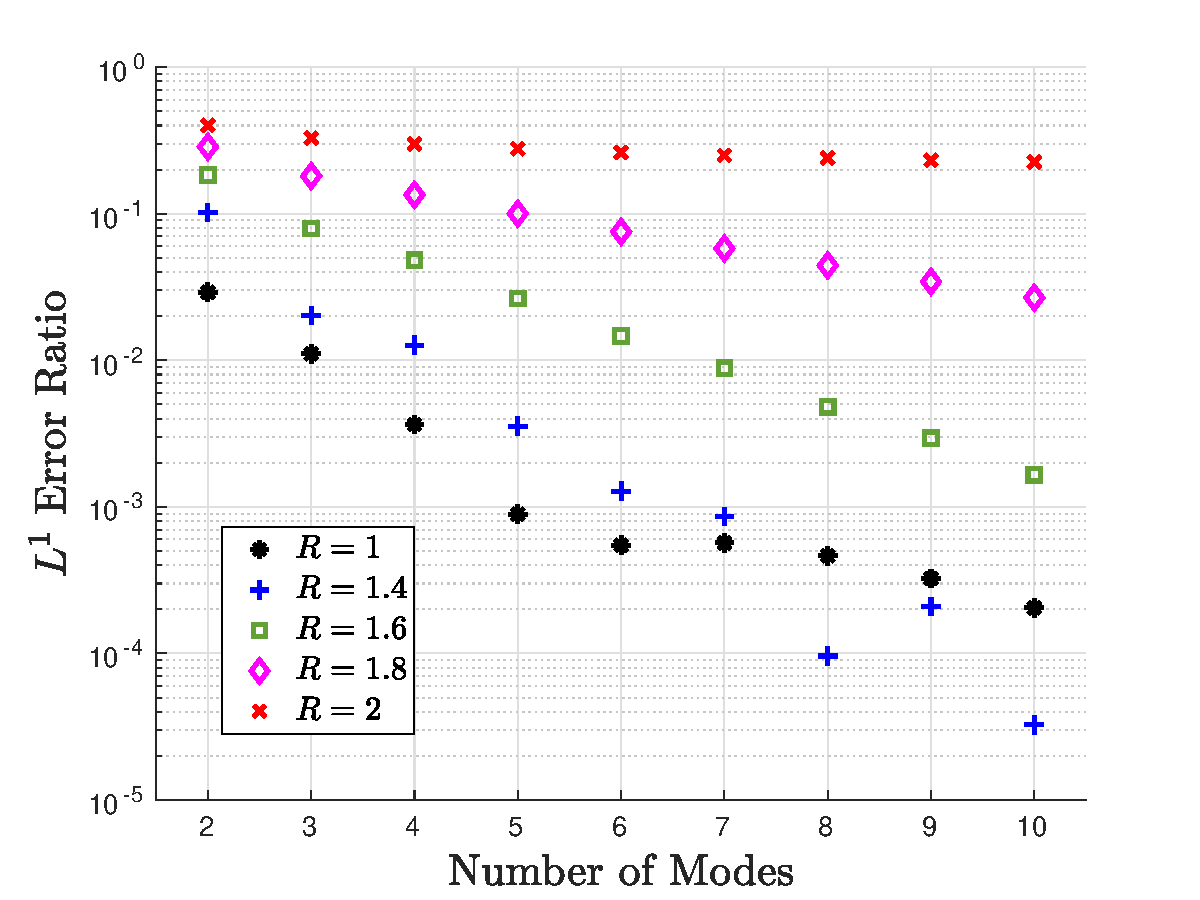
\includegraphics[width=0.8\linewidth]{plots/free_stream_f0_approx_Ups_5.pdf}}
\caption{Errors in expansion of \req{zerothApprox} as a function of number of modes, $\Upsilon=0.5$. \radapt{Birrell:2014gea}.}\label{fig:freeStreamf0approxUps5}
 \centerline{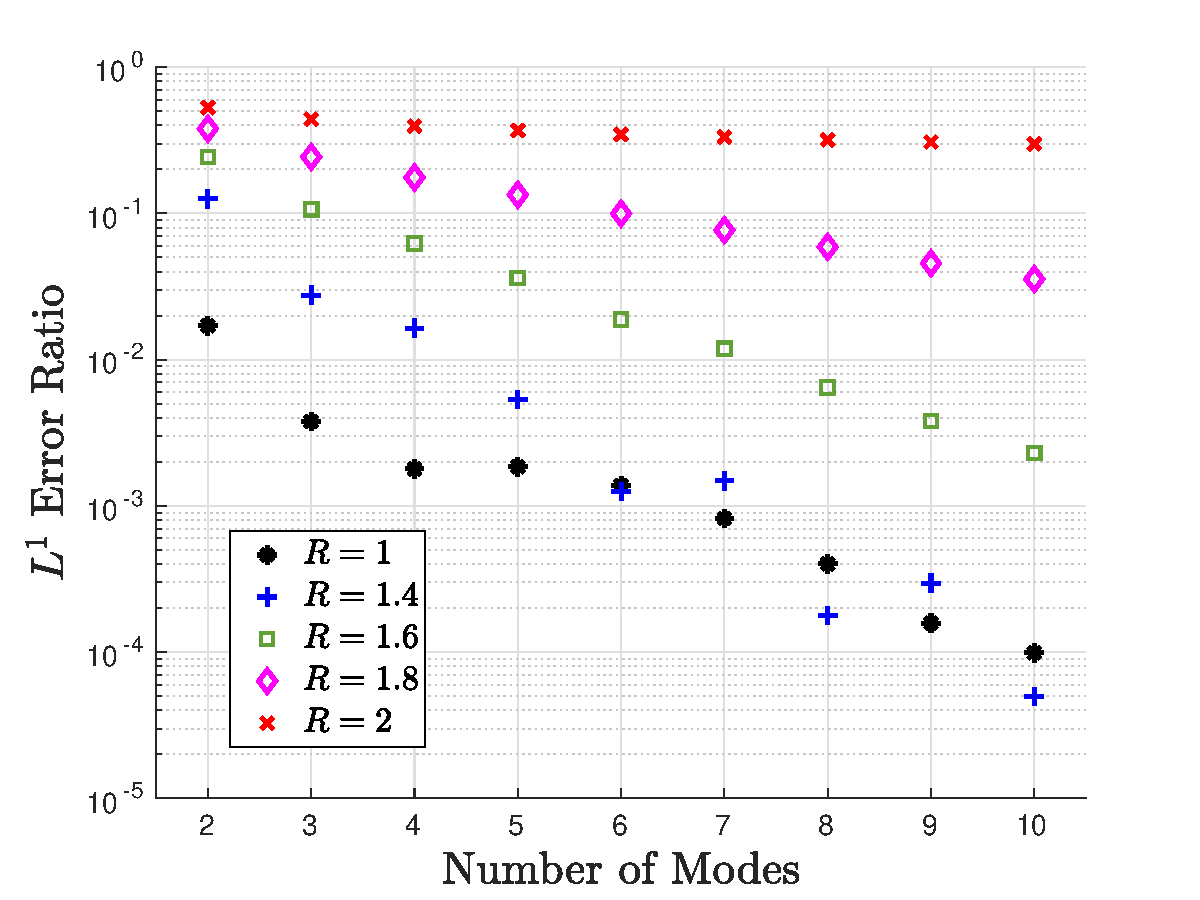
\includegraphics[width=0.8\linewidth]{plots/free_stream_f0_approx_Ups_1_5.pdf}}
\caption{Errors in  expansion of \req{zerothApprox} as a function of number of modes, $\Upsilon=1.5$. \radapt{Birrell:2014gea}.}\label{fig:freeStreamf0approxUps15}
\end{figure}
%%%%%%%%%%%%%%%%%%%%%%%%%%%%%%%%%%%%


We note the appearance of the reheating ratio
\begin{equation}\label{reheat}
 R\equiv aT  
\end{equation}
in the denominator of \req{zerothApprox}, which comes from changing variables from $z=p/T$ in \req{weight} to $y=ap$ in order to compare with \req{freeStreamWeight}.  Physically, $R$ is the ratio of the physical temperature $T$ to the dilution controlled temperature scaling  of $1/a$.   In physical situations, including cosmology, $R$ can vary from unity when dimensioned energy scales influence dynamical equations for $a$. From the error plots we see that for $R$ sufficiently close to $1$, the approximation performs well with a small number of terms, even with $\Upsilon\neq 1$.  




 In the case of large reheating, we find that when $R$ approaches and surpasses $2$, large spurious oscillations begin to appear in the expansion and they persist even when a large number of terms are used, as seen in Figures  \ref{fig:freeStreamf0approxUps1Tr185} and \ref{fig:freeStreamf0approxUps1Tr2}, where we compare $f_\Upsilon/f_{ch}^{1/2}$ with $f_{\Upsilon}^N/f_{ch}^{1/2}$ for $\Upsilon=1$ and $N=20$. See Ref.~\cite{Birrell:2014gea} for further discussion of the origin of these oscillations. This demonstrates that the chemical equilibrium method with dilution temperature scaling will  perform extremely poorly in situations that experience a large degree of reheating. For $R\approx 1$, the benefit of including fugacity is not as striking, as the chemical equilibrium basis is able to approximate \req{zerothApprox} reasonably well.  However, for more stringent error tolerances including $\Upsilon$ can reduce the number of required modes in cases, where the degree of chemical nonequilibrium is large.
%%%%%%%%%%%%%%%%%%%%%%%%%%%%%%%%%%%%%%%
\begin{figure}[ht]
\centerline{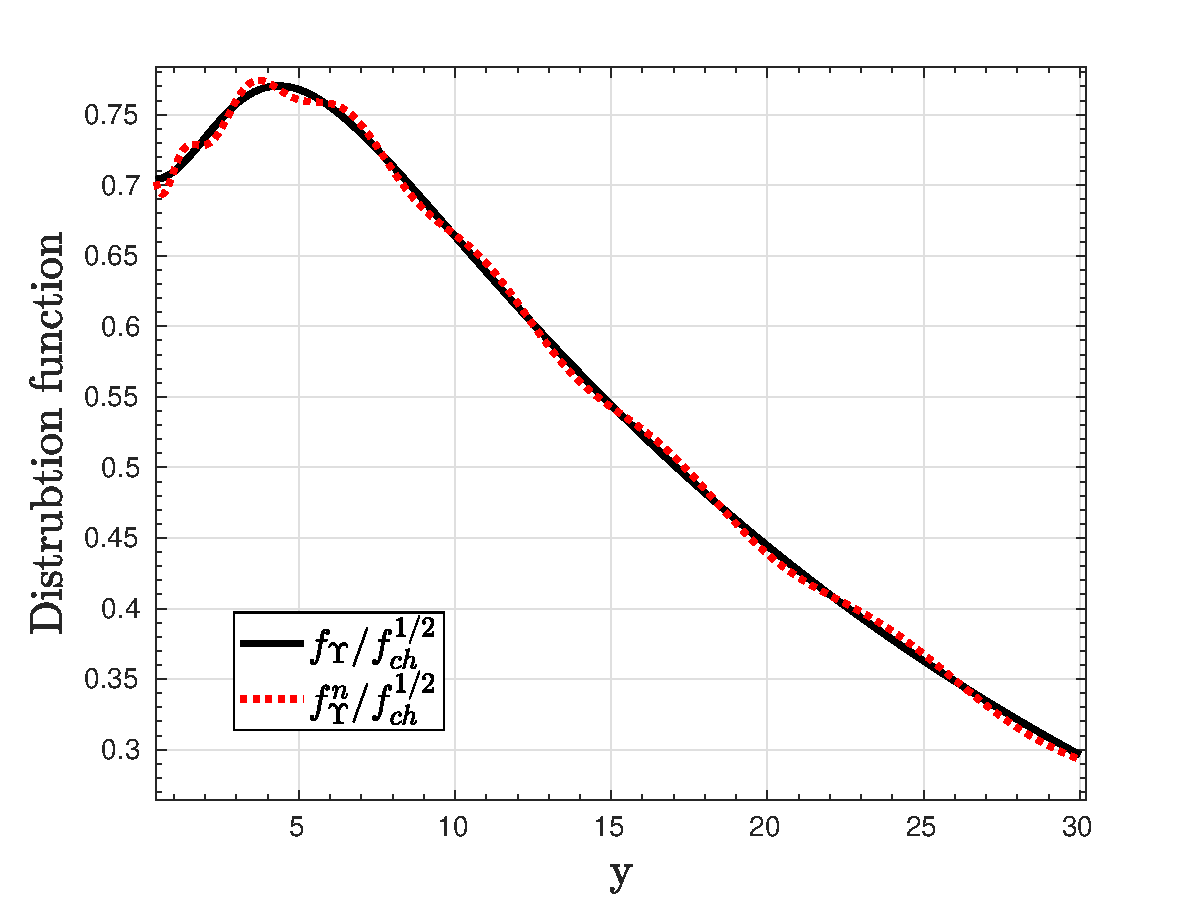
\includegraphics[width=0.8\linewidth]{plots/free_stream_f0_approx_Ups_1_T_r_1_85_n_20.pdf}}
\caption{Approximation to \req{zerothApprox} for $\Upsilon=1$ and $R=1.85$ using the first $20$ basis elements generated by \req{freeStreamWeight}. \radapt{Birrell:2014gea}.}\label{fig:freeStreamf0approxUps1Tr185}
 \centerline{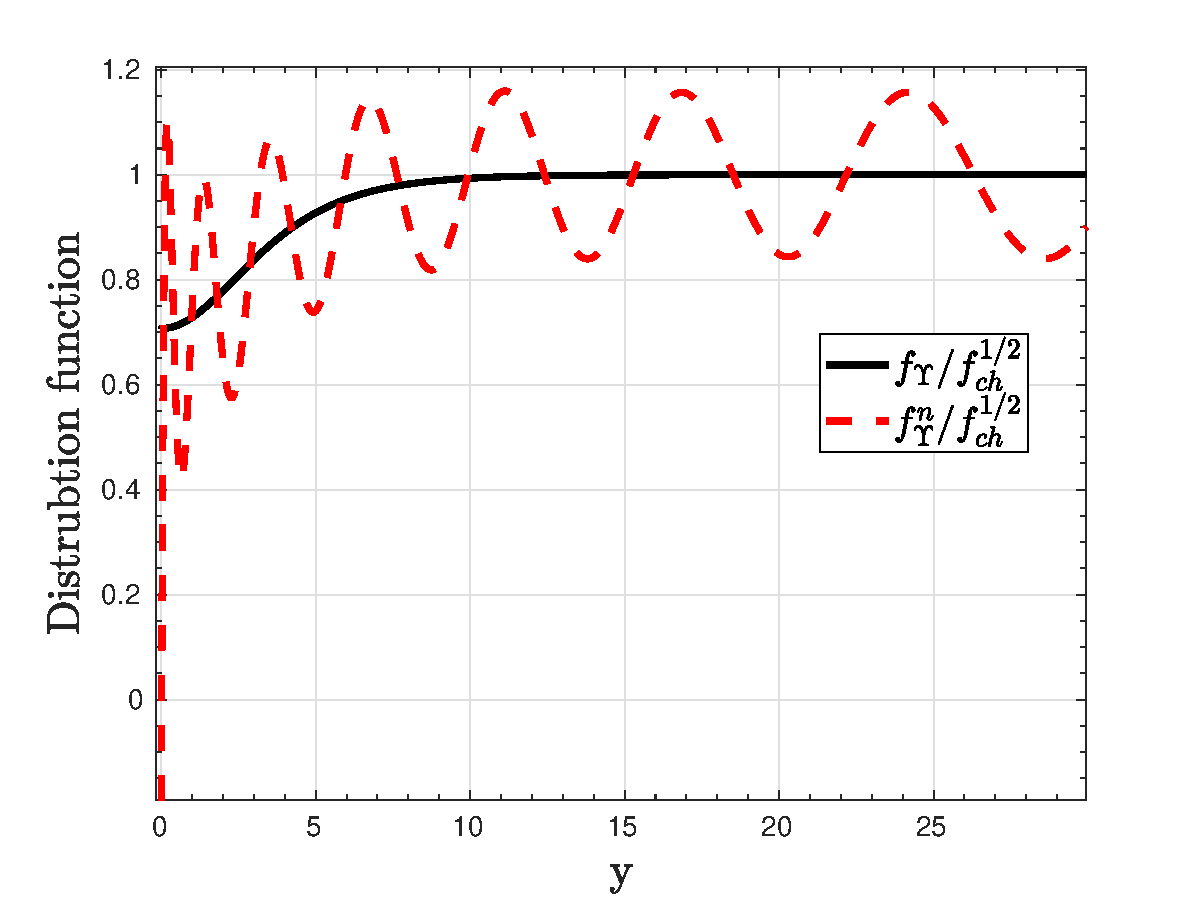
\includegraphics[width=0.8\linewidth]{plots/free_stream_f0_approx_Ups_1_T_r_2_n_20.pdf}}
\caption{Approximation to \req{zerothApprox} for $\Upsilon=1$ and $R=2$ using the first $20$ basis elements generated by \req{freeStreamWeight}. \radapt{Birrell:2014gea}.}\label{fig:freeStreamf0approxUps1Tr2}
\end{figure}
%%%%%%%%%%%%%%%%%%%%%%%%%%%%%%%%%%%%

%%%%%%%%%%%%%%%%%%%%%%%%%%%%%%%%%%%%%%%%%%%%%%%%%%%%%%%%%%%
\para{Nonequilibrium dynamics}\label{dynamicsSec}
In this section we derive the dynamical equations for the chemical nonequilibrium method. In particular, we identify physically motivated dynamics for the effective temperature and fugacity. Using \req{TBoltzmann} and the definition of $\psi$ from \req{kineticApprox} we have
\begin{align}\label{nearEquilibEq}
\partial_t \psi+\frac{1}{f_\Upsilon }\frac{\partial f_\Upsilon }{\partial\Upsilon}\dot\Upsilon\psi-\frac{z}{f_\Upsilon }\left(H+\frac{\dot{T}}{T}\right)\left(\psi\partial_zf_\Upsilon +f_\Upsilon \partial_z \psi\right)=\frac{1}{f_\Upsilon E}C[f_\Upsilon \psi]\,.
\end{align}
Denote the monic orthogonal polynomial basis generated by the weight, \req{weight}, by $\psi_n$, $n=0,1,...$, where $\psi_n$ is degree $n$ and call the normalized versions  $\hat{\psi}_n$. Recall that $\hat\psi_n$ depend on $t$ due to the $\Upsilon$ dependence of the weight function used in the construction; therefore the method developed here is a moving-frame spectral method. Consider the space of polynomial of degree less than or equal to $N$, spanned by $\hat\psi_n$, $n=0,...,N$.   For $\psi$ in this subspace, we expand $\psi=\sum_{j=0}^Nb^j\hat\psi_j$ and use \req{nearEquilibEq}  to obtain
\begin{align}\label{Tvars}
\sum_i \dot{b}^i\hat\psi_i=&\sum_ib^i\frac{z}{f_\Upsilon }\left(H+\frac{\dot{T}}{T}\right)\left(\partial_z(f_\Upsilon )\hat\psi_i+f_\Upsilon \partial_z\hat\psi_i\right)\\
&-\sum_ib^i\left(\dot{\hat{\psi}}_i+\frac{1}{f_\Upsilon }\frac{\partial f_\Upsilon }{\partial\Upsilon}\dot\Upsilon\hat\psi_i\right)+\frac{1}{f_\Upsilon E}C[f]\,.
\notag
\end{align}
From this we see  that  projecting the Boltzmann-Einstein equation onto the finite dimensional subspace gives
\begin{align}
\dot b^k=& \sum_i b^i\left(H+\frac{\dot{T}}{T}\right)\left(\langle\frac{z}{f_\Upsilon }\hat\psi_i\partial_zf_\Upsilon ,\hat\psi_k\rangle+\langle z\partial_z \hat\psi_i,\hat\psi_k\rangle\right) \\
&-\sum_i b^i\dot{\Upsilon}\left(\langle\frac{1}{f_\Upsilon }\frac{\partial f_\Upsilon }{\partial\Upsilon}\hat\psi_i,\hat\psi_k\rangle+\langle\frac{\partial\hat{\psi}_i}{\partial \Upsilon},\hat\psi_k\rangle\right)+\langle\frac{1}{f_\Upsilon E}C[f],\hat\psi_k\rangle\notag\,,
\end{align}
where $\langle\cdot,\cdot\rangle$ denotes the inner product defined by the weight function, \req{weight},
\begin{equation}
\langle h_1,h_2\rangle=\int_0^\infty h_1(z)h_2(z)w_\Upsilon(z)dz\,.
\end{equation}
The the collision term contains polynomial nonlinearities when multiple coupled distribution are being modeled using a $2$-$2$ collision operator, \req{coll}, while the other terms are linear.  

To isolate the linear part, we define matrices
\begin{align}\label{ABmatrices}
A^k_i(\Upsilon)\equiv&\langle\frac{z}{f_\Upsilon }\hat\psi_i\partial_zf_\Upsilon ,\hat\psi_k\rangle+\langle z\partial_z \hat\psi_i,\hat\psi_k\rangle\,,\\
B^k_i(\Upsilon)\equiv& C_i^k(\Upsilon)+D_i^k(\Upsilon),\hspace{2mm} C_i^k\equiv\Upsilon\langle\frac{1}{f_\Upsilon }\frac{\partial f_\Upsilon }{\partial\Upsilon}\hat\psi_i,\hat\psi_k\rangle,\hspace{2mm} D_i^k\equiv\Upsilon\langle\frac{\partial\hat{\psi}_i}{\partial \Upsilon},\hat\psi_k\rangle\,. \notag
\end{align}
 With these definitions, the equations for the $b^k$ become
\begin{align}\label{bEq}
\dot b^k=& \left(H+\frac{\dot{T}}{T}\right)\sum_i A_i^k(\Upsilon)b^i-\frac{\dot{\Upsilon}}{\Upsilon}\sum_i B_i^k(\Upsilon)b^i+\langle\frac{1}{f_\Upsilon E}C[f],\hat\psi_k\rangle\,.
\end{align}
 See  \rsec{sec:orthopolyApp} for details on how to recursively construct the $\partial_z\hat\psi_i$. We also showed how to compute the inner products $\langle\hat\psi_k,\partial_{\Upsilon}\hat\psi_k\rangle$.
 %in  Section \ref{ortho-polynom-fam}. 
 In  \req{eq:lowerTri1}-\req{eq:lowerTri5} we proved that that both $A$ and $B$ are lower triangular and show that the only inner products involving the $\partial_\Upsilon\hat{\psi}_i$ that are required in order to compute $A$ and $B$ are those the above mentioned diagonal elements, $\langle\hat\psi_k,\partial_{\Upsilon}\hat\psi_k\rangle$.


We fix the dynamics of $T$ and $\Upsilon$ by imposing the conditions
\begin{equation}\label{bIcs}
b^0(t)\hat\psi_0(t)=1\,,\hspace{2mm}b^1(t)=0\,.
\end{equation}
In other words,
\begin{equation}
f(t,z)=f_\Upsilon (t,z)\left(1+\phi(t,z)\right),\hspace{2mm} \phi=\sum_{i=2}^N b^i\hat\psi_i\,.
\end{equation}
This reduces the number of degrees of freedom in \req{bEq} from $N+3$ to $N+1$.  In other words, after enforcing \req{bIcs}, \req{bEq} constitutes $N+1$ equations for the remaining $N+1$ unknowns, $b^2,...,b^N$, $\Upsilon$, and $T$.  We will call $T$ and $\Upsilon$ the first two ``modes", as their dynamics arise from imposing the conditions \req{bIcs} on the zeroth and first order coefficients in the expansion. We will solve for their dynamics explicitly below.

To see the physical motivation for the choices \req{bIcs}, consider the particle number density and energy density.  Using the orthonormality of the $\hat\psi_i$ and \req{bIcs} we have
\begin{align}
n=&\frac{g_pT^3}{2\pi^2}\sum_ib^i\int_0^\infty f_\Upsilon  \hat\psi_i z^2 dz=\frac{g_pT^3}{2\pi^2}\sum_ib^i\langle \hat\psi_i ,1\rangle\\
=&\frac{g_pT^3}{2\pi^2}b^0\langle \hat\psi_0 ,1\rangle=\frac{g_pT^3}{2\pi^2}\langle 1 ,1\rangle\,,\notag\\
\rho=&\frac{g_pT^4}{2\pi^2}\sum_ib^i\int_0^\infty f_\Upsilon  \hat\psi_i z^3 dz=\frac{g_pT^4}{2\pi^2}\sum_ib^i\langle\hat\psi_i, z\rangle\\
=&\frac{g_pT^4}{2\pi^2}\left(b^0\langle\hat\psi_0, z\rangle+b^1\langle\hat\psi_1, z\rangle\right)=
\frac{g_pT^4}{2\pi^2}\langle 1,z\rangle\,.\notag
\end{align}
These, together with the definition of the weight function, \req{weight}, imply
\begin{align}\label{thEqMoments}
n=&\frac{g_pT^3}{2\pi^2}\int_0^\infty f_\Upsilon  z^2dz\,,\\
\label{thEqMoments2}
\rho=&\frac{g_pT^4}{2\pi^2}\int_0^\infty f_\Upsilon  z^3dz\,.
\end{align}
Equations (\ref{thEqMoments}) and (\ref{thEqMoments2}) show  that the first two modes, $T$ and $\Upsilon$, with time evolution fixed by \req{bIcs} cause the chemical nonequilibrium distribution $f_\Upsilon $ to capture the number density and energy density of the system exactly.  This fact is very significant, as it implies that within the chemical nonequilibrium approach as long as the back-reaction from the non-thermal distortions is small (meaning that the evolution of $T(t)$ and $\Upsilon(t)$ is not changed significantly when more modes are included), {\em all the effects relevant to the computation of  particle and energy flow are modeled by the time evolution of $T$ and $\Upsilon$ alone} and no further modes are necessary.  This gives a clear separation between the averaged physical quantities, characterized by $f_\Upsilon $, and the momentum dependent non-thermal distortions as captured by 
\begin{equation}
\phi=\sum_{i=2}^N b^i\hat\psi_i\,.
\end{equation}

One should contrast this chemical nonequilibrium behavior  with the chemical equilibrium method, where a minimum of four modes is required to describe the number and energy densities, as shown in \req{freeStreamMoments}.   Moreover we will show that convergence to the desired precision is faster in the chemical nonequilibrium approach as compared to chemical equilibrium. Due to the high cost of numerically integrating realistic collision integrals of the form \req{coll}, this fact can be very significant in applications. We remark that the relations \req{thEqMoments} are the physical motivation for including the $z^2$ factor in the weight function. All three modifications we have made in constructing our new method, the introduction of an effective temperature, i.e., $R\ne 1$, the generalization to chemical nonequilibrium $f_\Upsilon $, and the introduction of $z^2$ to the weight, \req{reheat}, were needed to obtain the properties, \req{thEqMoments}, but it is the introduction of $z^2$ that reduces the number of required modes and hence reduces the computational cost. 

With $b^0$ and $b^1$ fixed as in \req{bIcs} we can solve the equations for $\dot b^0$ and $\dot b^1$ from \req{bEq} for $\dot\Upsilon$ and $\dot T$ to obtain

\begin{align}\label{UpsTEqs}
\dot{\Upsilon}/{\Upsilon}=&\frac{(Ab)^1\langle\frac{1}{f_\Upsilon E}C[f],\hat\psi_0\rangle-(Ab)^0\langle\frac{1}{f_\Upsilon E}C[f],\hat\psi_1\rangle }{[\Upsilon\partial_\Upsilon \langle1,1\rangle/(2||\psi_0||)+(Bb)^0](Ab)^1-(Ab)^0(Bb)^1}\,,\\[0.5cm]
\dot{T}/T
=&\frac{(Bb)^1\langle\frac{1}{f_\Upsilon E}C[f],\hat\psi_0\rangle-\langle\frac{1}{f_\Upsilon E}C[f],\hat\psi_1\rangle[\Upsilon\partial_\Upsilon \langle1,1\rangle/(2||\psi_0||)+(Bb)^0]}{[\Upsilon\partial_\Upsilon \langle1,1\rangle/(2||\psi_0||)+(Bb)^0](Ab)^1-(Ab)^0(Bb)^1}-H\notag\\[0.3cm]
=&\frac{1}{(Ab)^1}\left((Bb)^1\dot{\Upsilon}/\Upsilon-\langle\frac{1}{f_\Upsilon E}C[f],\hat\psi_1\rangle\right)-H\,.\label{Teq}
\end{align}

Here $(Ab)^n=\sum_{j=0}^NA^n_jb^j$ and similarly for $B$ and $||\cdot||$ is the norm induced by $\langle\cdot,\cdot\rangle$. In deriving this, we used
\begin{equation}
\dot{b}^0=\frac{1}{2||\psi_0||}\dot\Upsilon\partial_\Upsilon \langle1,1\rangle\,, \hspace{4mm} \partial_\Upsilon \langle1,1\rangle=\int_0^\infty \frac{z^2}{(e^{z/2}+ \Upsilon e^{-z/2})^2}dz\,,
\end{equation}
which comes from differentiating \req{bIcs}. 
 
It is easy to check that when the collision operator vanishes, then the above system is solved by 
\begin{equation}\label{freeStreamSol}
\Upsilon=\text{constant}\,,\hspace{4mm} \frac{\dot T}{T}=-H\,,\hspace{2mm}  b^n=\text{constant}\,,\hspace{1mm} n>2\,,
\end{equation}
i.e., the fugacity and non-thermal distortions are `frozen' into the distribution and the temperature satisfies dilution scaling $T\propto 1/a$.

When the collision term becomes small, \req{freeStreamSol} motivates another change of variables. Letting $T=(1+\epsilon)/a$  gives the equation
\begin{equation}
\dot\epsilon=\frac{1+\epsilon}{(Ab)^1}\left((Bb)^1\dot{\Upsilon}/\Upsilon-\langle\frac{1}{f_\Upsilon E}C[f],\hat\psi_1\rangle\right).
\end{equation}
Solving this in place of \req{Teq} when the collision terms are small avoids having to numerically track the free-streaming evolution. In particular this will ensure conservation of comoving particle number, which equals a function of $\Upsilon$ multiplied by $(aT)^3$, to much greater precision in this regime as well as resolve the freeze-out temperatures more accurately.\\

%%%%%%%%%%%%%%%%%%%%%%%%%%%%%%%%%%%%%%%%%%%%%%%%%%%%%%%%%%
\noindent{\bf Projected Dynamics are Well-defined:}\\
The following calculation shows that, for a distribution initially in kinetic equilibrium, the determinant factor in the denominator of \req{UpsTEqs} is nonzero and hence the dynamics for $T$ and $\Upsilon$, as well as the remainder of the projected system, are well-defined, at least for sufficiently small times. 

Kinetic equilibrium\index{kinetic equilibrium} implies the initial conditions $b^0=||\psi_0||$, $b^i=0$, $i>0$.  Therefore we have
\begin{align}
K\equiv& (\Upsilon\partial_\Upsilon \langle 1,1\rangle/(2||\psi_0||)+(Bb)^0)(Ab)^1-(Ab)^0(Bb)^1\\[0.3cm]
=&(C^0_0A^1_0-A^0_0C^1_0)(b^0)^2+\left[(D^0_0A^1_0-A^0_0D^1_0)(b^0)^2+\Upsilon\partial_\Upsilon \langle 1,1\rangle/(2||\psi_0||)A^1_0b^0\right]\notag\\[0.3cm]
\equiv & K_1+K_2\,.\notag
\end{align}
\begin{align}
K_1=&\langle \frac{1}{1+\Upsilon e^{-z}},1\rangle\langle \frac{-z}{1+\Upsilon e^{-z}}\hat\psi_1,\hat\psi_0\rangle-\langle\frac{-z}{1+\Upsilon e^{-z}},\hat\psi_0\rangle\langle\frac{1}{1+ \Upsilon e^{-z}}\hat\psi_1,1\rangle\,.
\end{align}
Inserting the formula for $\hat\psi_1$ from \req{polyRecursion}, we find
\begin{align}
K_1=&-\frac{1}{||\psi_1||\,||\psi_0||}\left[\langle\frac{1}{1+ \Upsilon e^{-z}},\hat\psi_0\rangle\langle\frac{z^2}{1+\Upsilon e^{-z}},\hat\psi_0\rangle-\langle\frac{z}{1+\Upsilon e^{-z}},\hat\psi_0\rangle^2\right]\,.
\end{align}
The Cauchy-Schwarz inequality  applied to the inner product with weight function
\begin{equation}
\tilde{w}=\frac{w}{1+\Upsilon e^{-z}}\hat\psi_0
\end{equation}
together with linear independence of $1$ and $z$ implies that the term in brackets is positive and so $K_1<0$ at $t=0$.  For the second term, noting that $D^1_0=0$ by orthogonality and using \req{normDerivEq}, we have
\begin{align}
K_2=&[\langle\partial_\Upsilon\hat\psi_0,\hat\psi_0\rangle||\psi_0||+\partial_\Upsilon \langle 1,1\rangle/(2||\psi_0||)]\Upsilon A_0^1||\psi_0||=0\,.
\end{align}
This proves that $K$ is nonzero at $t=0$.\\

%%%%%%%%%%%%%%%%%%%%%%%%%%%%%%%%%%%%%%%%%%%%%
\subsection{Validation}\label{validation}
We will validate our numerical method on an exactly solvable model problem
\begin{equation}\label{toyEq}
\partial_t f-pH \partial_p f=M\left(\frac{1}{\Upsilon^{-1}e^{p/T_{eq}}+1}-f(p,t)\right)\,, \hspace{2mm} f(p,0)=\frac{1}{e^{p/T_{eq}(0)}+1}\,,
\end{equation}
where $M$ is a constant with units of energy and we choose units in which it is equal to $1$. This model describes a distribution that is attracted to a given equilibrium distribution at a prescribed time dependent temperature $T_{eq}(t)$ and fugacity\index{fugacity} $\Upsilon$. This type of an idealized scattering operator, without fugacity, was first introduced in \cite{Anderson:1974nyl}. By changing coordinates $y=a(t)p$ we find
\begin{equation}\label{freeStreamToy}
\partial_tf(y,t)=\frac{1}{\Upsilon^{-1}\exp[y/(a(t)T_{eq}(t))]+1}-f(y,t)\,,
\end{equation}
 which has as solution
\begin{equation}\label{exactSol}
f(y,t)=\int_0^t\frac{e^{s-t}}{\Upsilon^{-1}\exp[y/(a(s)T_{eq}(s))]+1}ds+\frac{e^{-t}}{\exp[y/(a(0)T_{eq}(0))]+1}\,.
\end{equation}
We now transform to $z=p/T(t)$, where the temperature $T$ of the distribution $f$ is defined as in Section \ref{dynamicsSec}.  Therefore, we have the exact solution to
\begin{equation}\label{kEqToy}
\partial_tf-z\left(H+\frac{\dot{T}}{T}\right)\partial_zf=\frac{1}{\Upsilon^{-1}e^{zT/T_{eq}}+1}-f(z,t)\,,
\end{equation}
given by
\begin{align}
f(z,t)=&\int_0^t\frac{e^{s-t}}{\Upsilon^{-1}\exp[a(t)T(t)z/(a(s)T_{eq}(s))]+1}ds\\
&+\frac{e^{-t}}{\exp[a(t)T(t)z/(a(0)T_{eq}(0))]+1}\,.\notag
\end{align}
We use this to test the chemical equilibrium and chemical nonequilibrium methods under two different conditions. 

%%%%%%%%%%%%%%%%%%%%%%%%%%%%%%%%%%%%%%%%%%%%%%%%%%%%%%%%%%%%%%%%%%%%%
\para{Reheating test}
First we compare the chemical equilibrium\index{chemical equilibrium} and nonequilibrium methods in a scenario that exhibits reheating.  Motivated by applications to cosmology, we choose a scale factor evolving as in the radiation dominated era, a fugacity $\Upsilon=1$, and choose an equilibrium temperature that exhibits reheating like behavior with $aT_{eq}$ increasing for a period of time,
\begin{align}\label{aTDef}
a(t)=\left(\frac{t+b}{b}\right)^{1/2}\,,\ \  \ \
T_{eq}(t)=\frac{1}{a(t)}\left(1+\frac{1-e^{-t}}{e^{-(t-b)}+1}(R-1)\right)\,,
\end{align}
where $R$ is the desired reheating ratio. Note that $(aT_{eq})(0)=1$ and $(aT_{eq})(t)\rightarrow R$ as $t\rightarrow\infty$. Qualitatively, this is reminiscent of the dynamics of neutrino freeze-out, but the range of reheating ratio for which we will test our method is larger than found there.

We solved \req{freeStreamToy} and \req{kEqToy} numerically using the chemical equilibrium and chemical nonequilibrium methods respectively for $t\in[0,10]$ and $b=5$ and the cases $R=1.1$, $R=1.4$, as well as the more extreme ratio of $R=2$.  The bases of orthogonal polynomials were generated numerically using the recursion relations from \rsec{sec:orthopolyApp}.  For the applications we are considering, where the solution is a small perturbation of equilibrium, only a small number of terms are required and so the numerical challenges associated with generating a large number of such orthogonal polynomials are not an issue.\\

%%%%%%%%%%%%%%%%%%%%%%%%%%%%%%%%%%%%%%%%%%%%%
\noindent{\bf Chemical equilibrium method}\\
We solved \req{freeStreamToy} using the chemical equilibrium method, with the orthonormal basis defined by the weight function \req{freeStreamWeight} for $N=2,...,10$ modes (mode numbers $n=0,...,N-1$) and prescribed  single step relative and absolute error tolerances of $10^{-13}$ for the numerical integration, and with asymptotic reheating ratios of $R=1.1$, $R=1.4$, and $R=2$.   

In  \rf{fig:freeStreamNumErr} and  \rf{fig:freeStreamEerr} we show the maximum relative error in the number densities and energy densities respectively over the time interval $[0,10]$ for various numbers of computed modes.  The particle number density and energy density are accurate, up to the integration tolerance level, for $3$ or more and $4$ or more modes respectively. This is consistent with \req{freeStreamMoments}, which shows the number of modes required to capture each of these quantities. However, fewer modes than these minimum values lead to a large error in the corresponding moment of the distribution function.
%%%%%%%%%%%%%%%%%%%%%%%%%%%%%%%%%%%%%%%
\begin{figure}
\centerline{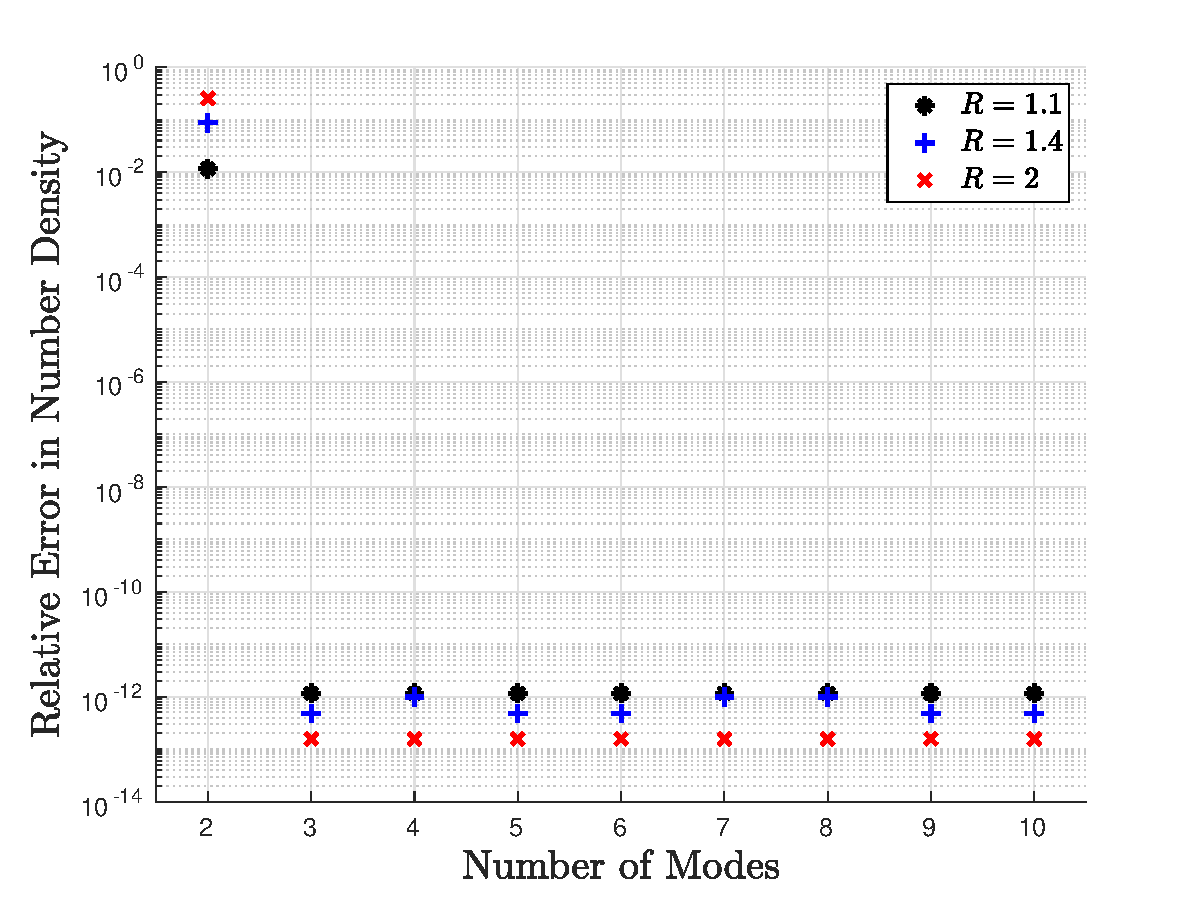
\includegraphics[width=0.8\linewidth]{plots/free_stream_num_err.pdf}}
\caption{Maximum relative error in particle number density. \radapt{Birrell:2014gea}.}\label{fig:freeStreamNumErr}
\centerline{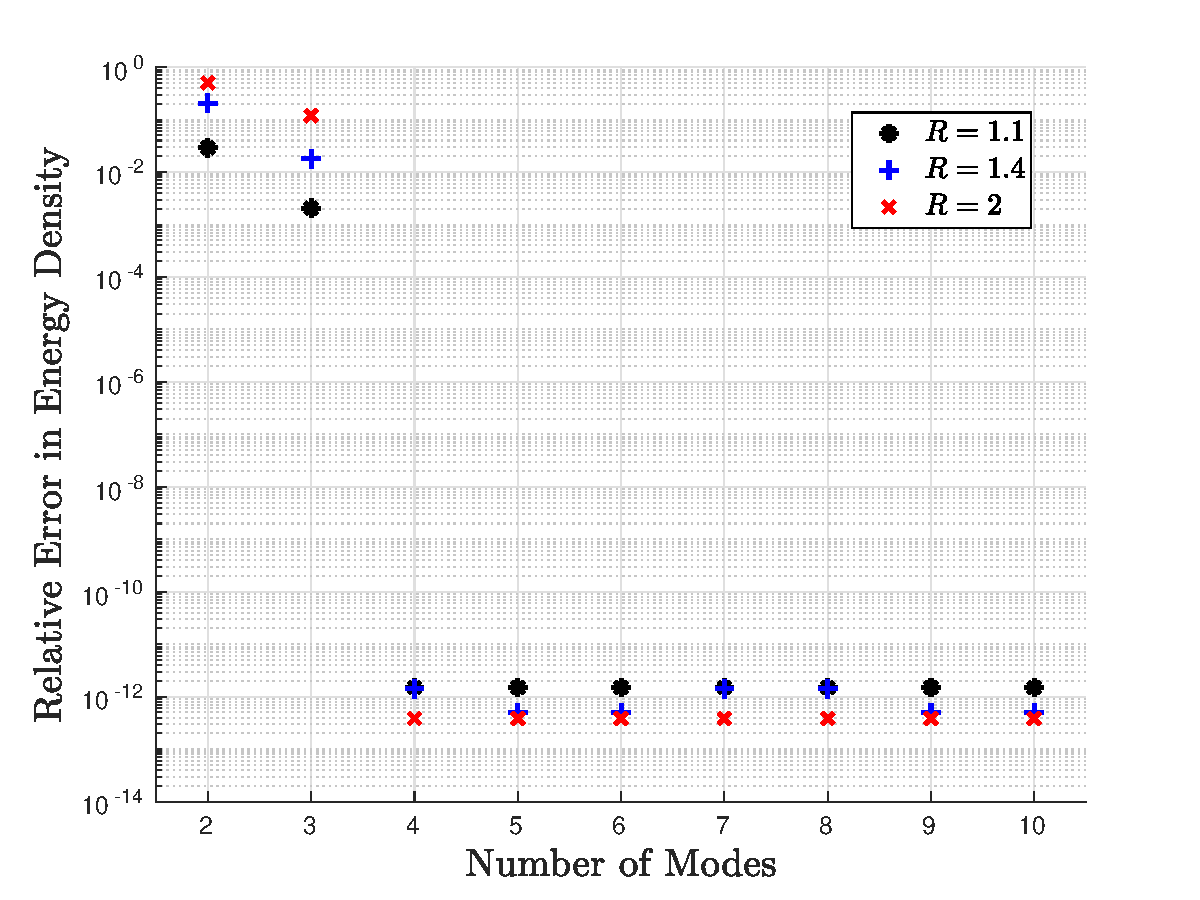
\includegraphics[width=0.8\linewidth]{plots/free_stream_E_err.pdf}}
\caption{Maximum relative error in energy density. \radapt{Birrell:2014gea}.}\label{fig:freeStreamEerr}
\end{figure}
%%%%%%%%%%%%%%%%%%%%%%%%%%%%%%%%%%%%%%%

%%%%%%%%%%%%%%%%%%%%%%%%%%%%%%%%%%%%%%%
\begin{figure}[ht]
\centerline{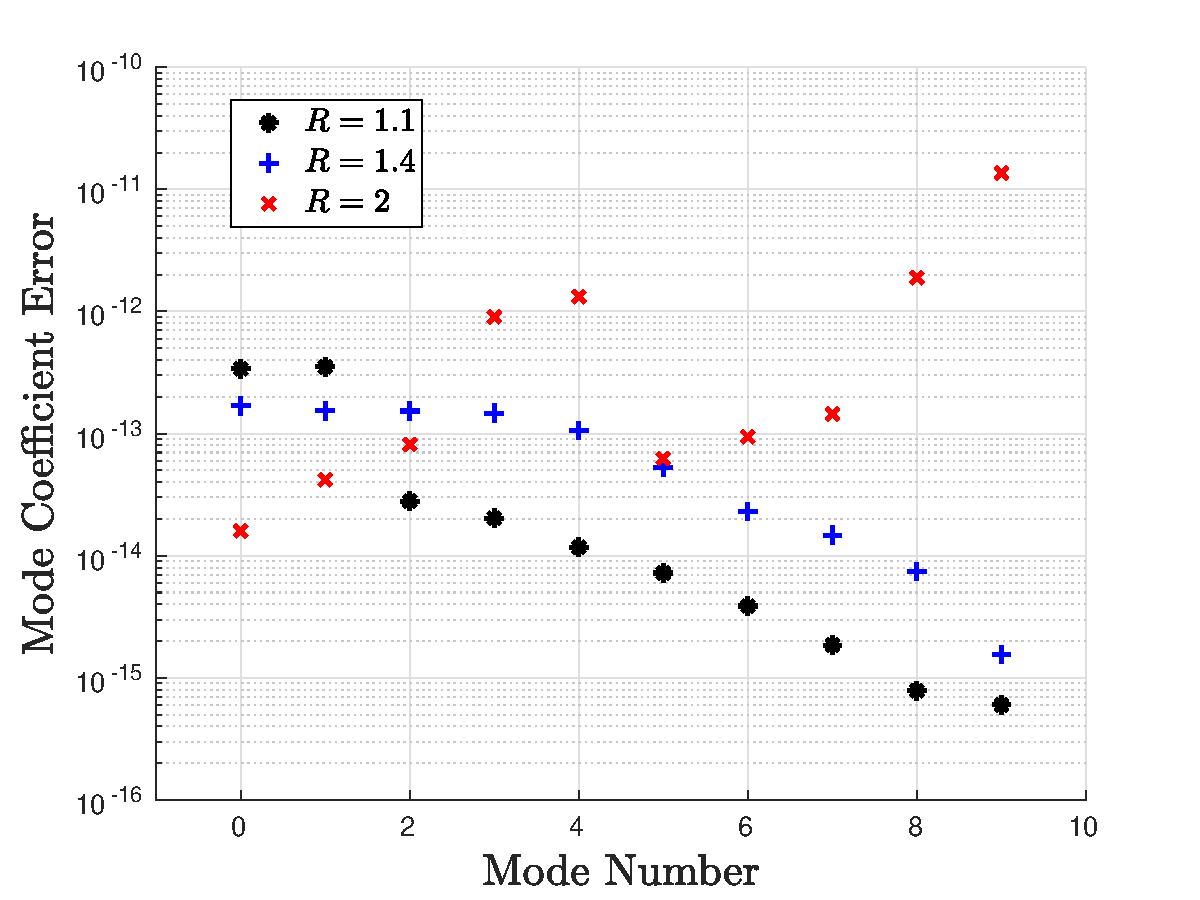
\includegraphics[width=0.8\linewidth]{plots/free_stream_b_err.pdf}}
\caption{Maximum error in mode coefficients. \radapt{Birrell:2014gea}.}\label{fig:freeStreambErr}
\centerline{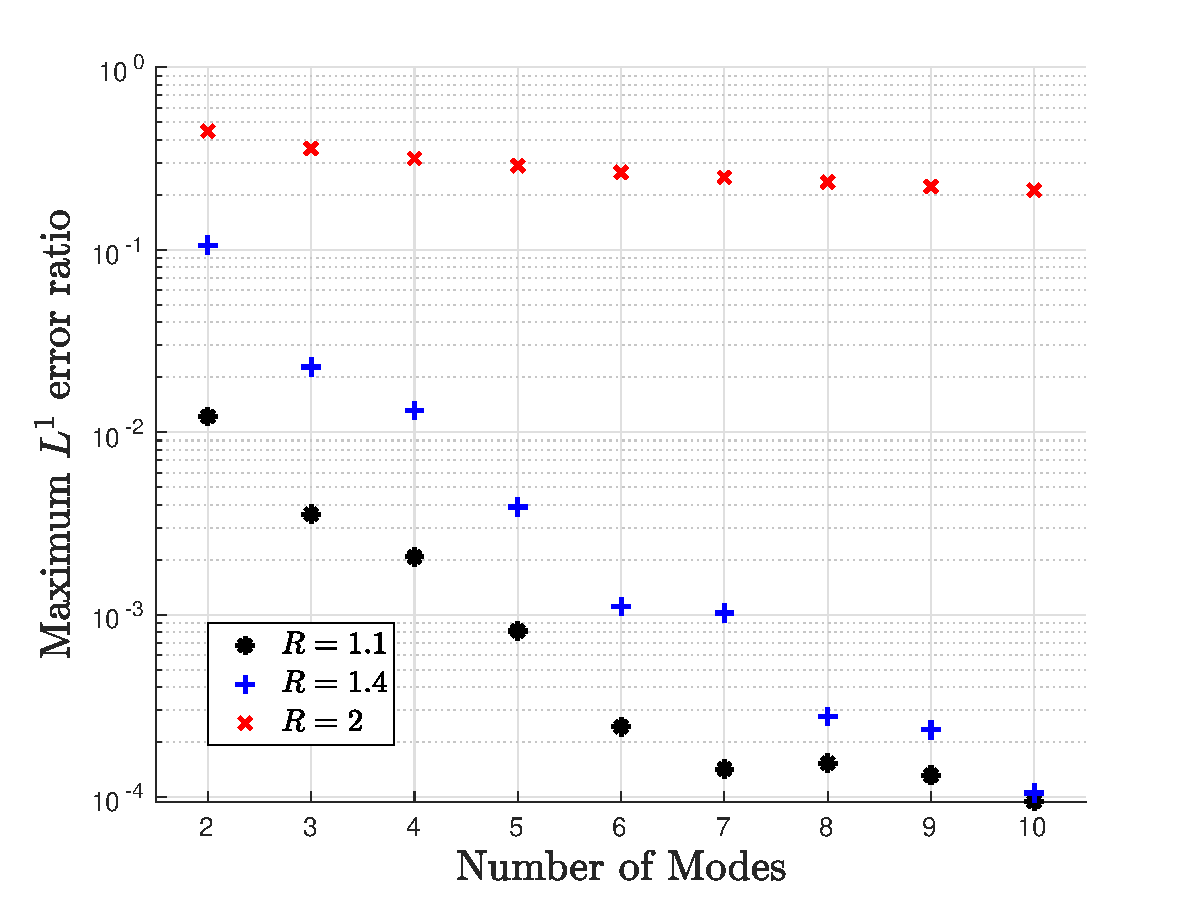
\includegraphics[width=0.8\linewidth]{plots/free_stream_L1_err.pdf}}
\caption{Maximum ratio  of $L^1$ error between computed and exact solutions to $L^1$ norm of the exact solution. \radapt{Birrell:2014gea}.}\label{fig:freeStreamL1Err}
\end{figure}
%%%%%%%%%%%%%%%%%%%%%%%%%%%%%%%%%%%%%%%

To show that the numerical integration accurately captures the mode coefficients of the exact solution, \req{exactSol}, in Figure \ref{fig:freeStreambErr} we show the error between the computed coefficients and actual coefficients, denoted by $\tilde b_n$ and $b_n$ respectively,
\begin{equation}\label{modeErrDef}
\text{error}_n=\max_{t} |\tilde{b}_n(t)-b_n(t)|\,,
\end{equation}
 where the evolution of the system was computed using $N=10$ modes.



In Figure  \ref{fig:freeStreamL1Err} we show the error between the exact solution $f$, and the numerical solution $f^N$ computed using $N=2,...,10$ modes over the solution time interval, where we define the error by
\begin{equation}\label{fErr}
\text{error}_N=\max_{t} \frac{\int |f-f^N|dy}{\int |f|dy}\,.
\end{equation}
%%%%%%%%%%%%%%%%%%%%%%%%%%%%%%%%%%%%%%%
\begin{figure}[ht]
\centerline{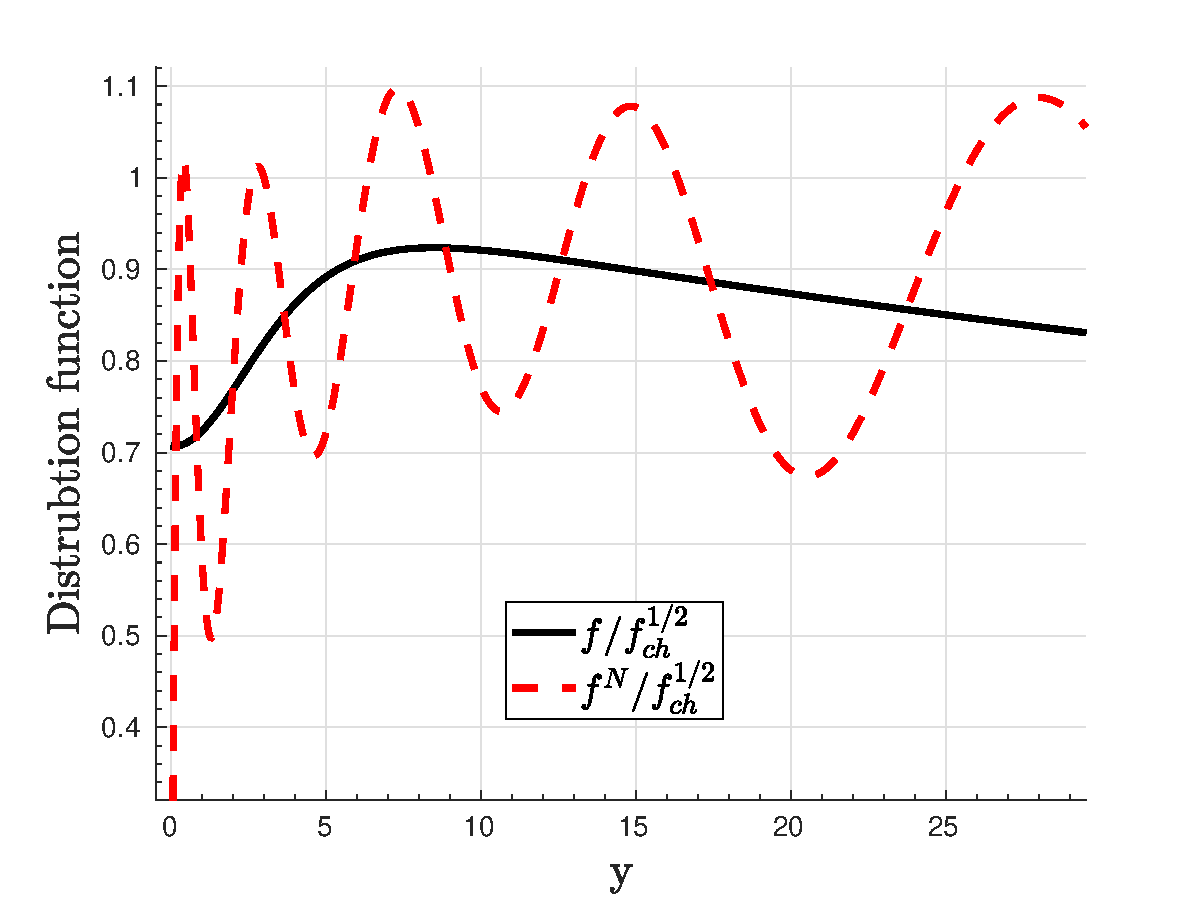
\includegraphics[width=0.8\linewidth]{plots/free_stream_approx_T_r_2.pdf}}
\caption{Approximate and exact solution for a reheating ratio $R=2$ and $N=10$ modes. \radapt{Birrell:2014gea}.}\label{fig:freeStreamApproxTr2}
 \centerline{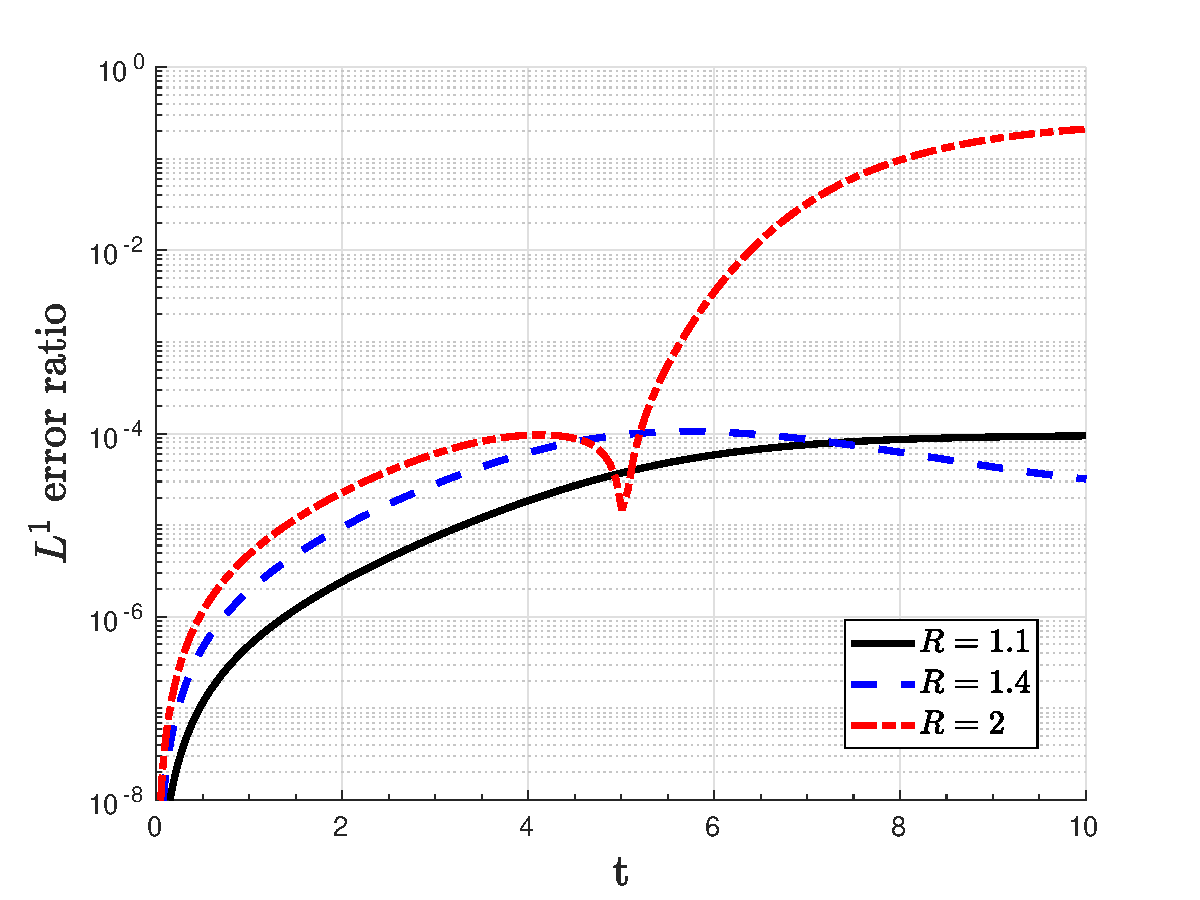
\includegraphics[width=0.8\linewidth]{plots/free_stream_L1_err_time.pdf}}
\caption{$L^1$ error ratio as a function of time for $N=10$ modes. \radapt{Birrell:2014gea}.}\label{fig:freeStreamL1errTime}
\end{figure}
%%%%%%%%%%%%%%%%%%%%%%%%%%%%%%%%%%%%%%%
For $R=1$ and $R=1.4$  the chemical equilibrium method works reasonably well (as long as the number of modes is at least 4, so that the energy and number densities are properly captured) but for $R=2$ the approximate solution exhibits spurious oscillations, as seen in Figure \ref{fig:freeStreamApproxTr2}, and has significantly degraded $L^1$ error;  this behavior is expected based on the results we did present earlier in this Appendix.
%in Section \ref{basisComparison}. 
Further clarifying the behavior, in Figure \ref{fig:freeStreamL1errTime}  we show the $L^1$ error ratio as a function of time for $N=10$ modes. In the $R=2$ case we see that the error increases as the reheating ratio approaches its asymptotic value of $R=2$ as $t\rightarrow\infty$.  As we will see, our methods achieves a much higher accuracy for a small number of terms in the case of large reheating ratio due to the replacement of dilution temperature scaling with the dynamical effective temperature $T$.\\ 

%%%%%%%%%%%%%%%%%%%%%%%%%%%%%%%%%%%%%%%%%%%%%%
\noindent{\bf Chemical non-equilibrium method}\\
We now solve  \req{freeStreamToy} using the chemical nonequilibrium method, with the orthonormal basis defined by the weight function, \req{weight}, for $N=2,...,10$ modes, a prescribed numerical integration tolerance of $10^{-13}$, and asymptotic reheating ratios of $R=1.1$, $R=1.4$, and $R=2$.  Recall that we are referring to $T$ and $\Upsilon$ as the first two modes ($n=0$ and $n=1$). 
%%%%%%%%%%%%%%%%%%%%%%%%%%%%%%%%%%%%%%%
\begin{figure}[ht]
\centerline{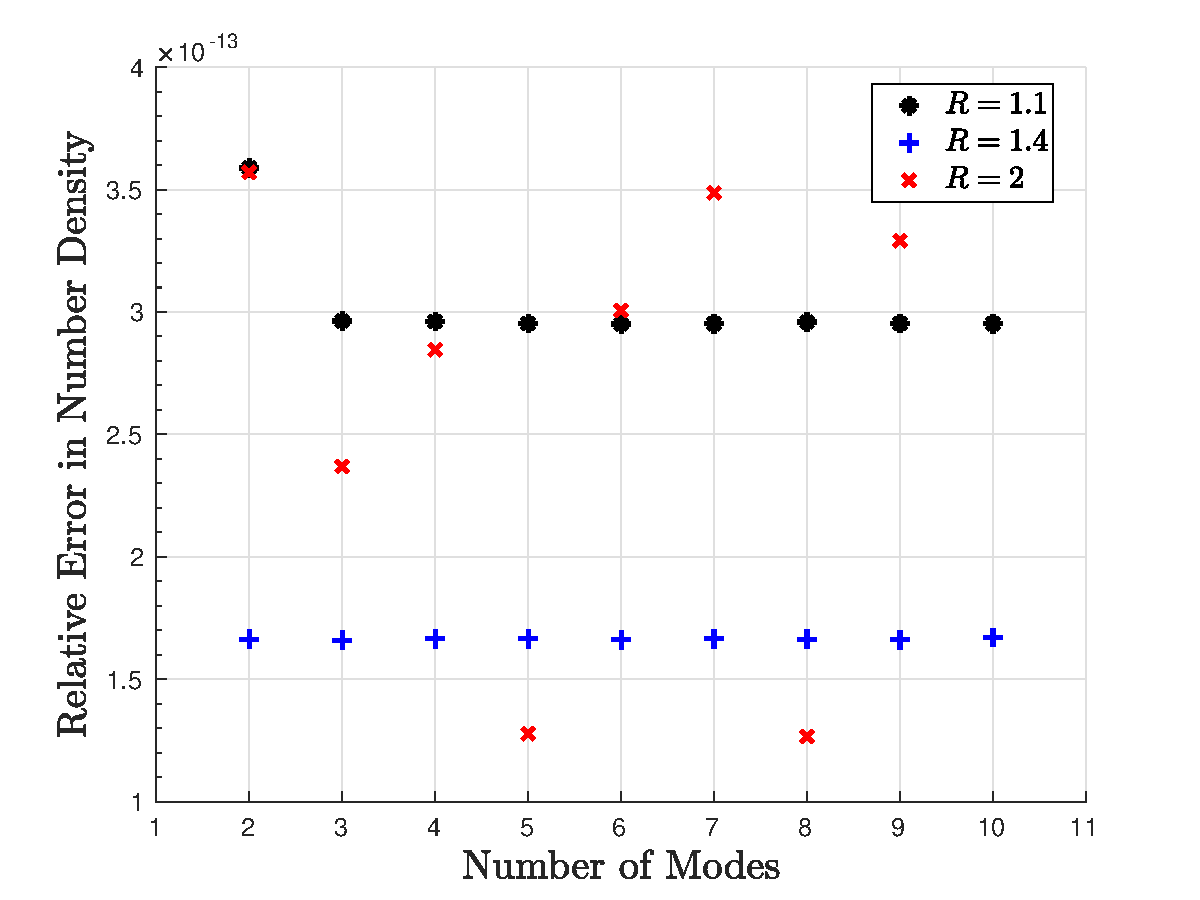
\includegraphics[width=0.9\linewidth]{plots/keq_num_err.pdf}}
\caption{Maximum relative error in particle number density. \radapt{Birrell:2014gea}.}\label{fig:keqNumErr}
 \centerline{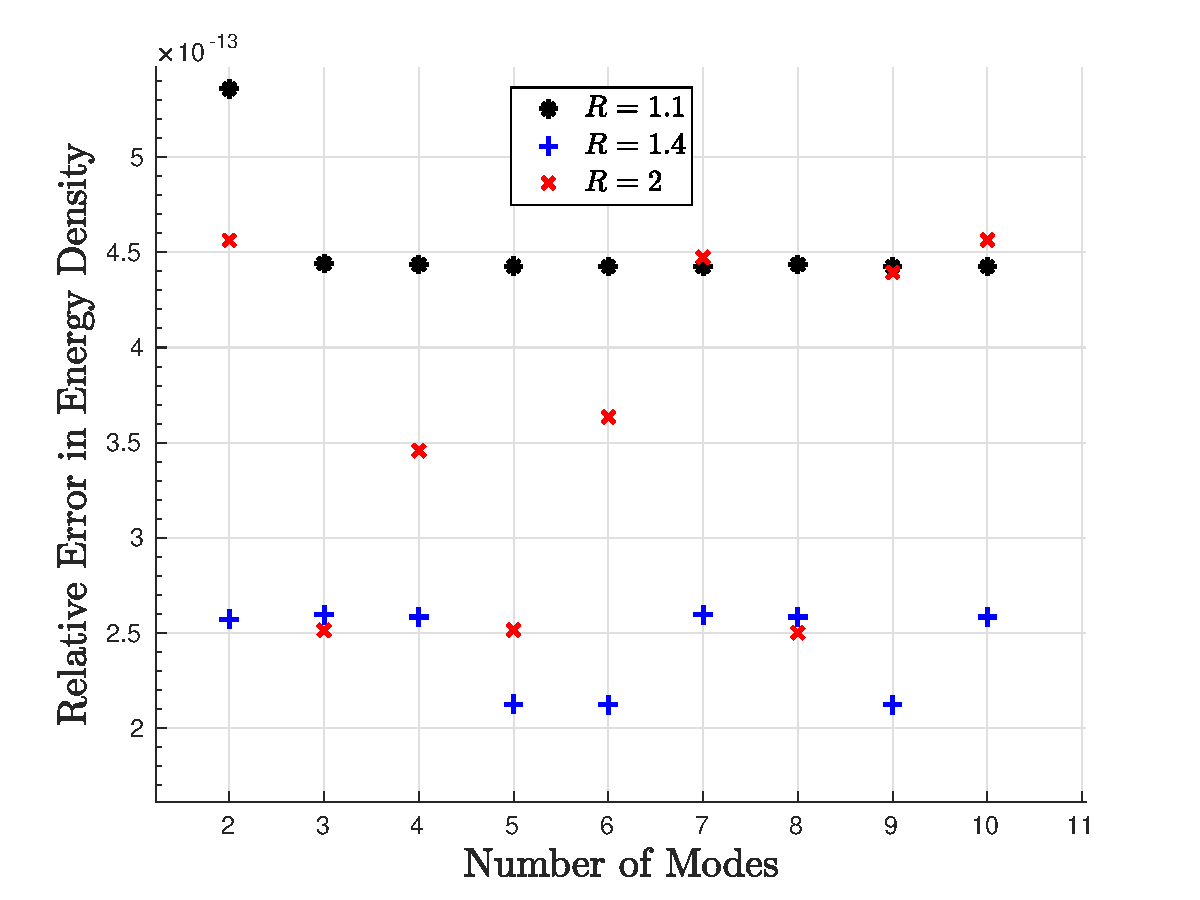
\includegraphics[width=0.9\linewidth]{plots/keq_E_err.pdf}}
\caption{Maximum relative error in energy density. \radapt{Birrell:2014gea}.}\label{fig:keqEerr}
\end{figure}
%%%%%%%%%%%%%%%%%%%%%%%%%%%%%%%%%%%%%%%
In Figures \ref{fig:keqNumErr} and  \ref{fig:keqEerr} we show the maximum relative error over the time interval $[0,10]$ in the number densities and energy densities respectively for various numbers of computed modes. Even for only $2$ modes, the number and energy densities are accurate up to the integration tolerance level.  This is in agreement with the analytical expressions in \req{thEqMoments}.



%%%%%%%%%%%%%%%%%%%%%%%%%%%%%%%%%%%%%%%
\begin{figure}[ht]
\centerline{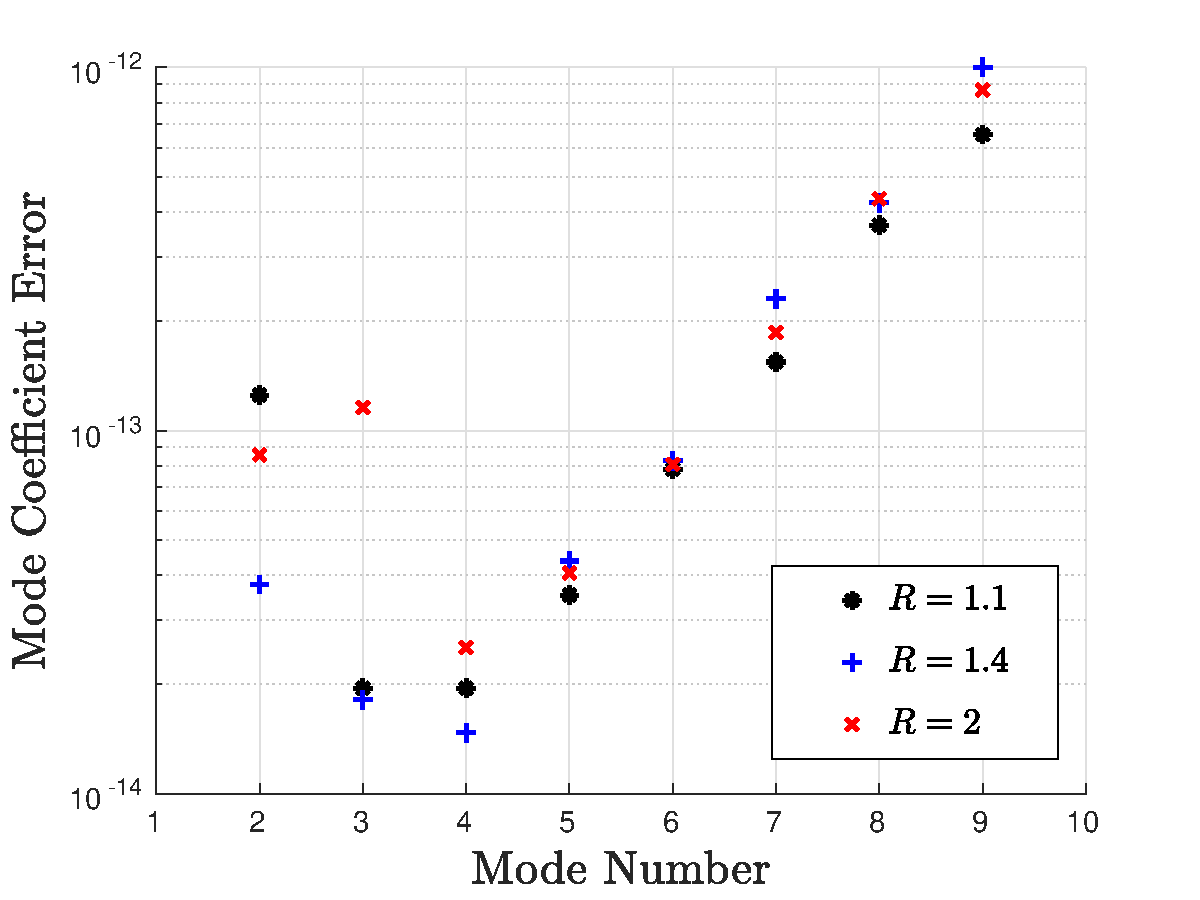
\includegraphics[width=0.9\linewidth]{plots/keq_b_err.pdf}}
\caption{Maximum error in mode coefficients. \radapt{Birrell:2014gea}.}\label{fig:keqbErr}
\centerline{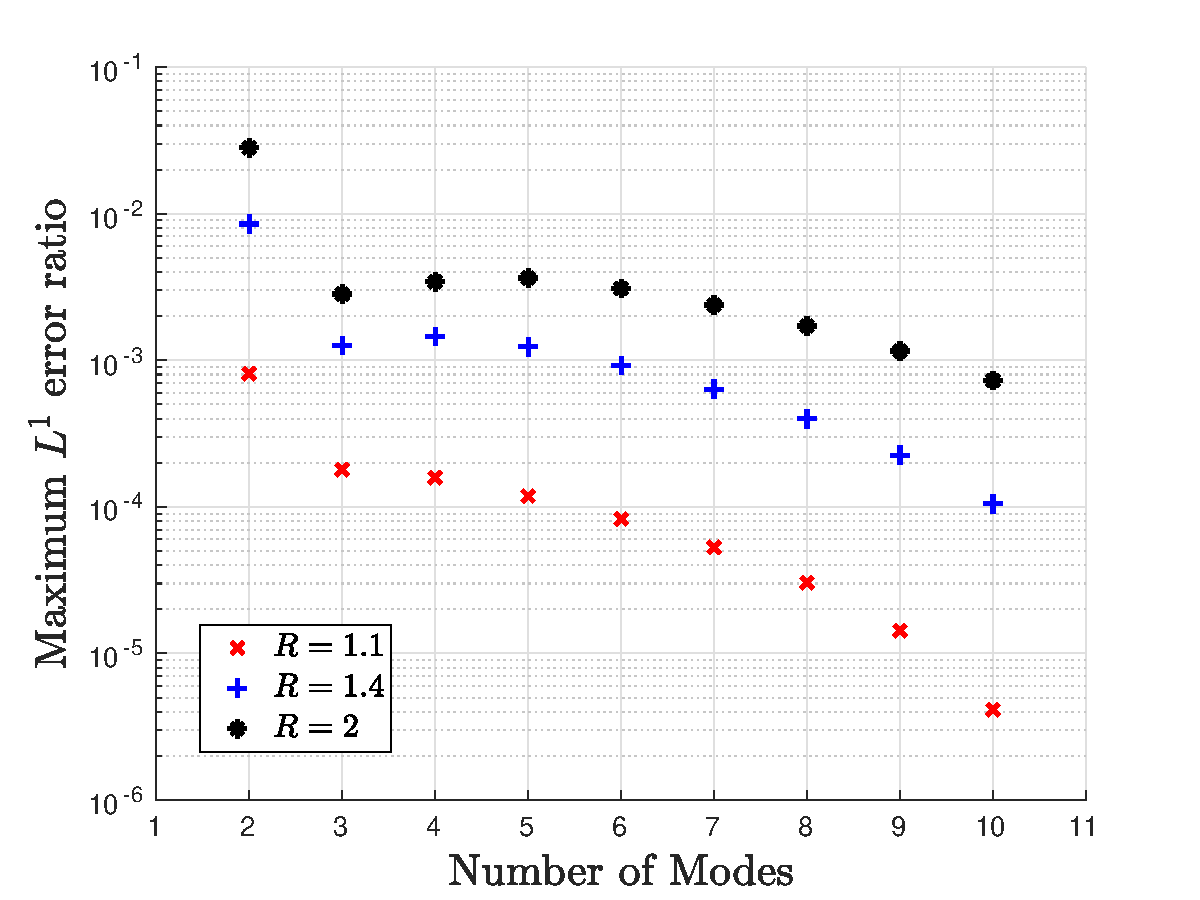
\includegraphics[width=0.9\linewidth]{plots/keq_L1_err.pdf}}
\caption{Maximum ratio of $L^1$ error between computed and exact solutions to $L^1$ norm of the exact solution. \radapt{Birrell:2014gea}.}\label{fig:keqL1Err}
\end{figure}
%%%%%%%%%%%%%%%%%%%%%%%%%%%%%%%%%%%%%%%


To show that the numerical integration accurately captures the mode coefficients of the exact solution, \req{exactSol}, in Figure \ref{fig:keqbErr} we show the error in the computed mode coefficients \req{modeErrDef}, where the evolution of the system was computed using $N=10$ modes. In Figure \ref{fig:keqL1Err} we show the error between the approximate and exact solutions, computed as in \req{fErr} for $N=2,...,10$ and $R=1.1$, $R=1.4$, and $R=2$ respectively.  For most mode numbers and $R$ values, the error using $2$ modes is substantially less than the error from the chemical equilibrium\index{chemical equilibrium} method using $4$ modes.  The result is most dramatic for the case of large reheating, $R=2$, where the spurious oscillations from the chemical equilibrium solution are absent in our method, as seen in Figure \ref{fig:keqApproxTr2}, as compared to the chemical equilibrium method in Figure \ref{fig:freeStreamApproxTr2}.  Note that we plot from $z\in [0,15]$ in comparison to $y\in[0,30]$ in Figure \ref{fig:keqApproxTr2} due to the relation $z=y/R$ as discussed in before in this Appendix. 
%Section \ref{basisComparison}. 
Additionally, the error no longer increases as $t\rightarrow\infty$, as it did for the chemical equilibrium method, see Figure \ref{fig:keqL1errTime}.  In fact it decreases since the exact solution approaches chemical equilibrium at a reheated temperature and hence can be better approximated by $f_\Upsilon$. 

In summary, in addition to the reduction in the computational cost when going from $4$ to $2$ modes, we also reduce the error compared to the chemical equilibrium method, all while accurately capturing the number and energy densities. 

%%%%%%%%%%%%%%%%%%%%%%%%%%%%%%%%%%%%%%%
\begin{figure}[ht]
\centerline{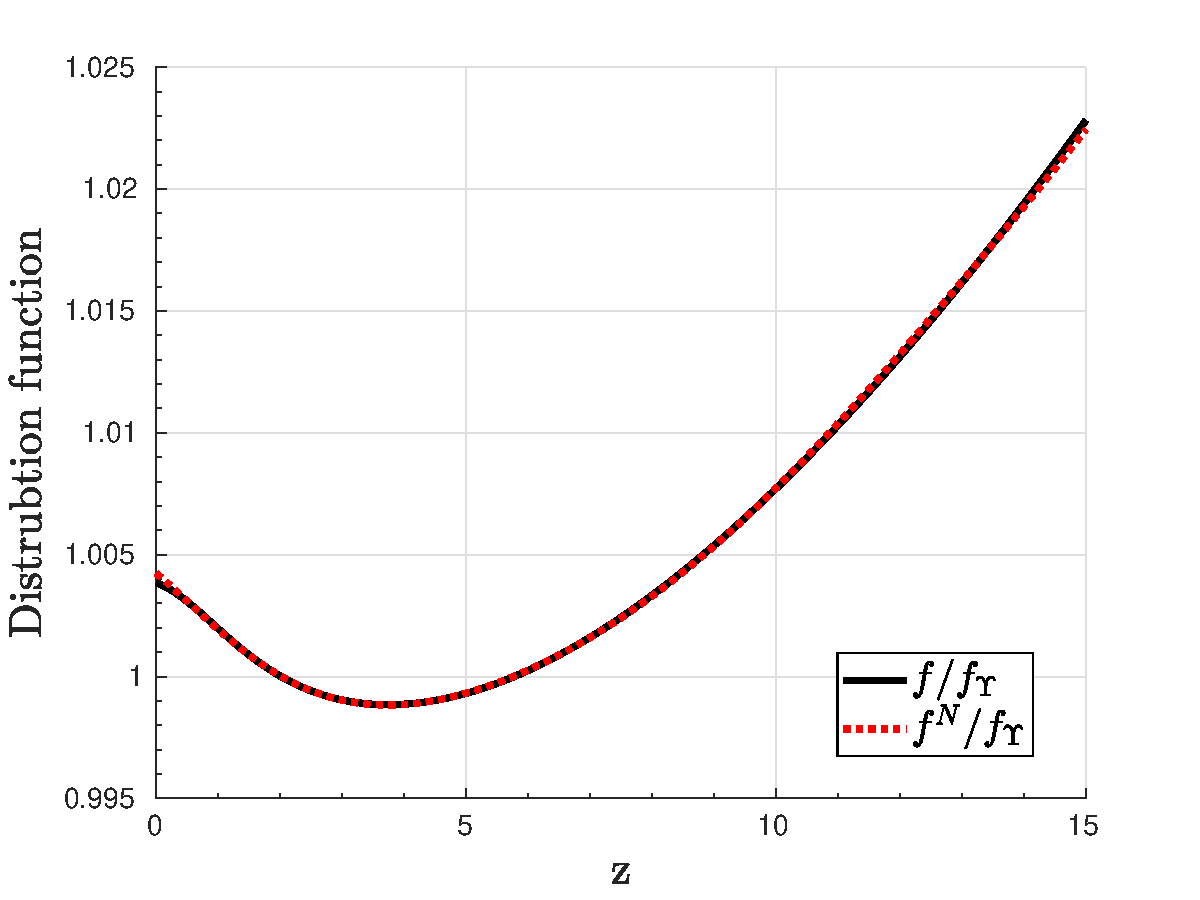
\includegraphics[width=0.9\linewidth]{plots/keq_approx_T_r_2.pdf}}
\caption{Approximate and exact solution for $R=2$ obtained with two modes. \radapt{Birrell:2014gea}.}\label{fig:keqApproxTr2}
\centerline{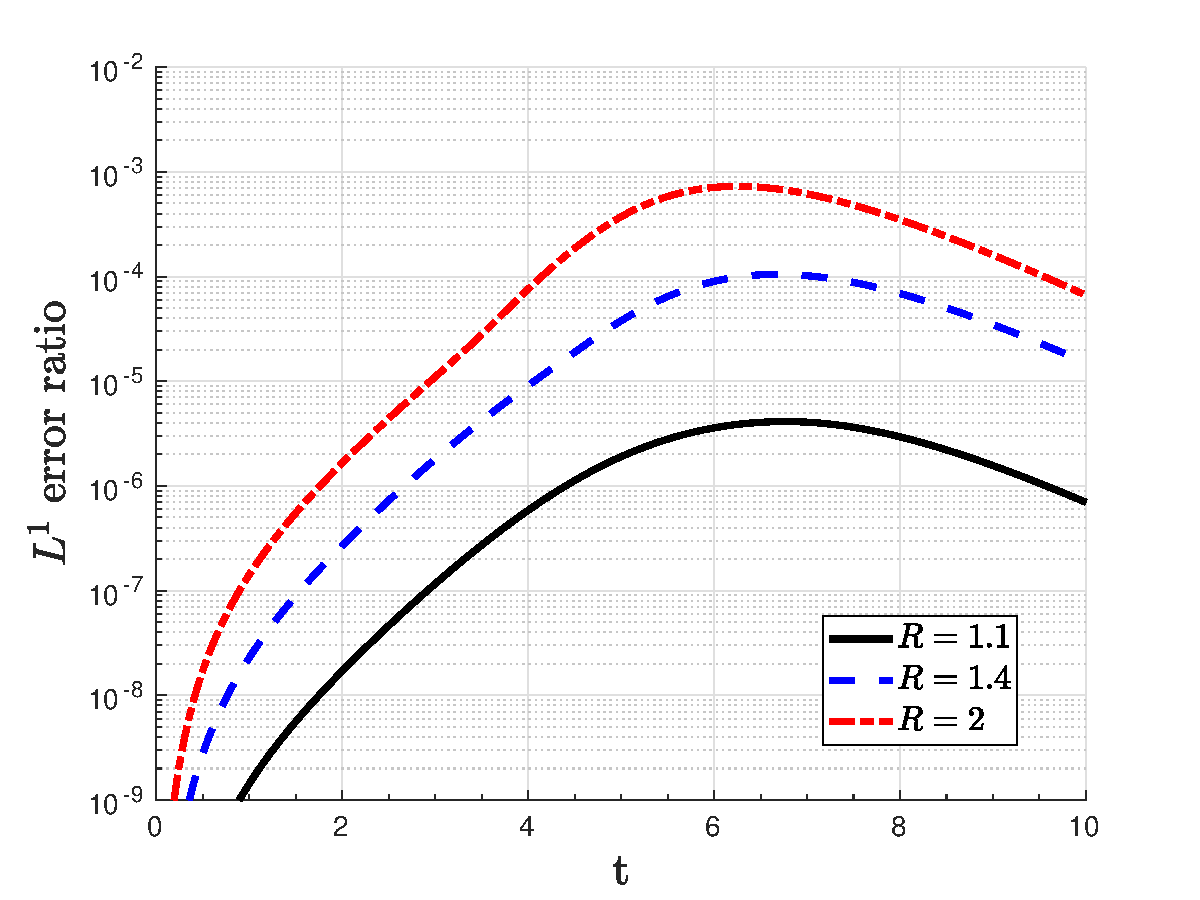
\includegraphics[width=0.9\linewidth]{plots/keq_L1_err_time.pdf}}
\caption{$L^1$ error ratio as a function of time for $n=10$ modes. \radapt{Birrell:2014gea}.}\label{fig:keqL1errTime}
\end{figure}
%%%%%%%%%%%%%%%%%%%%%%%%%%%%%%%%%%%%%%%
\clearpage